 \documentclass[oneside,a4paper,12pt]{book}
%\pagestyle{headings}
\frontmatter

%=============================================================================

\usepackage{amsthm}
\usepackage{xspace}
\usepackage{float}
\usepackage{ifthen}
\usepackage{amsbsy}
\usepackage{amssymb}
\usepackage{balance}
\usepackage{booktabs}
\usepackage{graphicx}
\usepackage{rotating}
\usepackage{multirow}
\usepackage{needspace}
\usepackage{microtype}
\usepackage{bold-extra}
\usepackage{geometry}
\usepackage{varioref}
\usepackage{xcolor}
\usepackage{textcomp}
\usepackage{listings}
\usepackage[normalem]{ulem} %emphasize still italic
\usepackage{ucs}

% \usepackage[utf8]{inputenc}
% \usepackage[htt]{hyphenat}
\usepackage{times}
\usepackage{url}
\usepackage{alltt}
\usepackage{amsmath}
\usepackage{xfrac}
\usepackage{subfigure}
\usepackage{appendix}
\usepackage{stmaryrd}   % for the \shortuparrow
\usepackage[utopia]{quotchap}

\usepackage{setspace}
\usepackage[numbers, sort&compress]{natbib}
\usepackage{mdwlist}        % support for better spaced lists
% allows for temporary adjustment of side margins
\usepackage{chngpage}
\usepackage[normalem]{ulem} 

% lina entered
\usepackage{indentfirst}
\usepackage[parfill]{parskip}
\usepackage[bottom]{footmisc}

\usepackage[T1]{fontenc}
\usepackage{caption}
\usepackage{booktabs}
\usepackage{siunitx}


\setlength{\parindent}{1.5em}

% constants

\newcounter{qcounter}

% commands
\newcommand{\n}{$\cdot$}
\newcommand{\y}{\checkmark}
\newcommand{\subscript}[1]{$_{\textrm{\footnotesize{#1}}}$}
\newcommand{\superscript}[1]{$^{\textrm{\footnotesize{#1}}}$}
\newcommand{\vertical}[1]{\raisebox{-4em}{\begin{sideways}{#1}\end{sideways}}}
\newcommand\tab[1][1cm]{\hspace*{#1}}

\usepackage{boxedminipage}

\newboolean{showedits}
\setboolean{showedits}{true} % toggle to show or hide edits
\ifthenelse{\boolean{showedits}}
{
       \newcommand{\ugh}[1]{\textcolor{red}{\uwave{#1}}} % please rephrase
       \newcommand{\ins}[1]{\textcolor{blue}{\uline{#1}}} % please insert
       \newcommand{\del}[1]{\textcolor{red}{\sout{#1}}} % please delete
       \newcommand{\chg}[2]{\textcolor{red}{\sout{#1}}{\ra}\textcolor{blue}{\uline{#2}}} % please change
}{
       \newcommand{\ugh}[1]{#1} % please rephrase
       \newcommand{\ins}[1]{#1} % please insert
       \newcommand{\del}[1]{} % please delete
       \newcommand{\chg}[2]{#2}
}


% ============================================================================
% Put edit comments in a really ugly standout display

\usepackage{xcolor}
\usepackage[normalem]{ulem}
\newcommand{\ra}{$\rightarrow$}
\usepackage{amssymb}

% comments \nb{label}{color}{text}
\newboolean{showcomments}
\setboolean{showcomments}{true}
%\setboolean{showcomments}{false}
\ifthenelse{\boolean{showcomments}}
{\newcommand{\nb}[3]{
  {\colorbox{#2}{\bfseries\sffamily\scriptsize\textcolor{white}{#1}}}
  {\textcolor{#2}{\sf\small$\blacktriangleright$\textit{#3}$\blacktriangleleft$}}}
    \newcommand{\version}{\emph{\scriptsize$-$Id$-$}}
%	 \newcommand{\ugh}[1]{\textcolor{red}{\uwave{#1}}} % please rephrase
%	 \newcommand{\ins}[1]{\textcolor{blue}{\uline{#1}}} % please insert
%	 \newcommand{\del}[1]{\textcolor{red}{\sout{#1}}} % please delete
%	 \newcommand{\chg}[2]{\textcolor{red}{\sout{#1}}{\ra}\textcolor{blue}{\uline{#2}}} % please change
	 \newcommand{\chk}[1]{\textcolor{ForestGreen}{#1}} % changed, please check
	}
{\newcommand{\nb}[3]{}
  \newcommand{\version}{}
  \newcommand{\chk}[1]{} % changed, please check
  }
\newcommand\nm[1]{\nb{NM}{violet}{#1}} % add more author macros here
\newcommand\lt[1]{\nb{LT}{orange}{#1}}


% ============================================================================
% Make quotes be italic
\renewenvironment{quote}
    {\list{}{\rightmargin\leftmargin}%
     \item\relax\begin{it}}
    {\end{it}\endlist}

\newcommand{\ttimes}{\ensuremath{\times}}

%=============================================================================

\newcommand{\needlines}[1]{\Needspace{#1\baselineskip}}

% source code
\usepackage{xcolor}
\usepackage{textcomp}
\usepackage{listings}
\definecolor{javared}{rgb}{0.6,0,0} % for strings
\definecolor{javagreen}{rgb}{0.25,0.5,0.35} % comments
\definecolor{javapurple}{rgb}{0.5,0,0.35} % keywords
\definecolor{javadocblue}{rgb}{0.25,0.35,0.75} % javadoc

\renewcommand{\lstlistingname}{Code}% Listing -> Algorithm
\renewcommand{\lstlistlistingname}{List of \lstlistingname s}% List of Listings -> List of Algorithms

\lstnewenvironment{Java}[1][]
{\lstset{
	language=Java,
	basicstyle=\footnotesize\ttfamily,
	keywordstyle=\color{javapurple}\bfseries,
	stringstyle=\color{javared},
	commentstyle=\color{javagreen},
	morecomment=[s][\color{javadocblue}]{/**}{*/},
	numbers=left,
	numberstyle=\tiny\color{black},
	stepnumber=1,
	numbersep=10pt,
	tabsize=4,
	showspaces=false,
	showstringspaces=false,
	breaklines=true,
	captionpos=b,
	xleftmargin=2em,
	framexleftmargin=1.5em,
	frame=single,
	#1
}}
{}


\lstnewenvironment{JVMIS}[1][]
{\lstset{
	language=JVMIS,
	basicstyle=\footnotesize\ttfamily,
	keywordstyle=\color{javagreen}\bfseries,
	stringstyle=\color{javared},
	commentstyle=\color{javagreen},
	morecomment=[s][\color{javadocblue}]{/**}{*/},
	numbers=none,
	numberstyle=\tiny\color{black},
	stepnumber=1,
	numbersep=10pt,
	tabsize=4,
	showspaces=false,
	showstringspaces=false
	breaklines=true,
	captionpos=b,
	xleftmargin=2em,
	framexleftmargin=1.5em,
	frame=single,
	#1
}}
{}


\definecolor{codegray}{gray}{0.9}
\newcommand{\code}[1]{
	\colorbox{codegray}
	{\texttt{#1}}
}

%----------------------------------------------------------------------------
% references
\newcommand{\tabref}[1]{\hyperref[{tab:#1}]{Table~\ref*{tab:#1}}}
\newcommand{\figref}[1]{\hyperref[{fig:#1}]{Figure~\ref*{fig:#1}}}
\newcommand{\secref}[1]{\hyperref[{sec:#1}]{Section~\ref*{sec:#1}}}
\newcommand{\subsecref}[1]{\hyperref[{subsec:#1}]{Subsection~\ref*{subsec:#1}}}
\newcommand{\lstref}[1]{\hyperref[{lst:#1}]{Listing~\ref*{lst:#1}}}
\newcommand{\charef}[1]{\hyperref[{ch:#1}]{Chapter~\ref*{ch:#1}}}
\newcommand{\coderef}[1]{\hyperref[{code:#1}]{Code~\ref*{code:#1}}}
\newcommand{\bytecoderef}[1]{\hyperref[{bytecode:#1}]{Bytecode~\ref*{bytecode:#1}}}
\newcommand{\algref}[1]{\hyperref[{alg:#1}]{Algorithm~\ref*{alg:#1}}}
\newcommand{\boxref}[1]{\hyperref[{box:#1}]{Box~\ref*{box:#1}}}

%----------------------------------------------------------------------------

% abbreviations
\tracingcolors 4
\setcounter{tocdepth}{3}
\setcounter{secnumdepth}{3}
\newcommand{\ie}{\emph{i.e.,}\xspace}
\newcommand{\eg}{\emph{e.g.,}\xspace}
\newcommand{\etc}{\emph{etc.}\xspace}
\newcommand{\etal}{\emph{et al.}\xspace}


\newcommand{\newevenside}{
	\ifthenelse{\isodd{\thepage}}{\newpage}{
	\newpage
        \phantom{placeholder} % doesn't appear on page
	\thispagestyle{empty} % if want no header/footer
	\newpage
	}
}

\def\stretchfactor{1}
\newcommand{\mychapter}[1]{\setstretch{1}
    \chapter{#1}\setstretch{\stretchfactor}}

%----------------------------------------------------------------------------
\newcommand{\lessSpace}{\vspace{-1em}}
\DeclareGraphicsExtensions{.pdf,.png}
\graphicspath{{images/}}
\newcommand{\fig}[4]{
	\begin{figure}[#1]
		\centering
		\includegraphics[width=#2\textwidth]{#3}
		\lessSpace
		\caption{\label{fig:#3}#4}
	\end{figure}}

% ===========================================================================

%:CONFIGURE THIS

\newcommand{\thesistitle}{Where does this null come from ?}
\newcommand{\thesisauthor}{Lina Tran}
\newcommand{\thesisauthorOrigin}{Biel/Bienne BE, Switzerland}
\newcommand{\thesisleiter}{Prof.\ Dr.\ Oscar Nierstrasz}
\newcommand{\thesisasst}{	\begin{center}
														Research assistant Nevena Milojkovi\'{c}\\
														Research assistant Boris Spasojevi\'{c}
													\end{center}}
\newcommand{\thesisurl}{http://scg.unibe.ch/}
\newcommand{\thesissubtitle}{An Approach to show the exact location where a value was referenced to null}
\newcommand{\thesisdate}{31. July 2016}

% ===========================================================================

\usepackage[ colorlinks=true, urlcolor=black, linkcolor=black,
			citecolor=black, bookmarksnumbered=true, bookmarks=true,
			plainpages=false,
			pdftitle={\thesistitle}, pdfauthor={\thesisauthor},
			pdfsubject={\thesissubtitle}, pdfpagelabels]{hyperref}

\newcommand{\hrref}[2]{\hyperref}
% ===========================================================================
% ===========================================================================


% D O C U M E N T
% % % % % % % % % % % % % % % % % % % % % % % % % % % % % % % % % %
\begin{document}

% T I T L E
% % % % % % % % % % % % % % % % % % % % % % % % % % % % % % % % % %
\begin{titlepage}  
  \begin{center}  
  
  \begin{figure}[t]  
  \vspace*{-2cm}        % to move header logo at the top 
  \center{
\includegraphics[scale=0.5]{logos/UNI_Bern.png}}
  \vspace{1in}     
  \end{figure}

    \thispagestyle{empty}
    
    {\bfseries\Huge \thesistitle \par
    \Large \vspace{0.1in} \thesissubtitle \par}

    \vspace{0.3in} 
    \LARGE{\textbf{Bachelor Thesis} \\}
    \vspace{0.4in}

    {\Large \thesisauthor \par from \par \thesisauthorOrigin}
    
    \vspace{0.3in}
    {\Large Faculty of Science \\
            University of Bern \par}
    \vspace{0.3in}
    {\Large \thesisdate \par}
    \vspace{0.3in}
    %Leiter der Arbeit: \par
   {\Large \thesisleiter} \par
      {\Large \thesisasst} \par
   \vspace{0.1in}
    {\Large Software Composition Group \par Institute for Computer Science \par University of Bern, Switzerland \par}
  

  %\vspace{0.5in}
 
 

  \end{center}

\end{titlepage}


% A B S T R A C T
% % % % % % % % % % % % % % % % % % % % % % % % % % % % % % % % % %
\chapter*{\centering Abstract}
\begin{quotation}
\noindent 
A previous study found out that \npe are the most frequently occurring and difficult to debug exceptions in Java projects. They are difficult to debug because the developer is only provided with a stack trace to where the exception was thrown. This only gives insight into the effect of the fault but not into its cause.

The aim of the project is to provide the developer with an additional stack trace of where the variable that caused the \npe was actually set to null. We attempt to achieve this goal by instrumenting java source code striving for a minimal execution overhead. 

By tracking the null assignments through static analysis and instrumentation of the bytecode we can achieve a more efficient debugging process after an occurrence of a \npe. 
\end{quotation}
\clearpage


% C O N T E N T S 
% % % % % % % % % % % % % % % % % % % % % % % % % % % % % % % % % % % % % % % %
\tableofcontents

\mainmatter
%%%%%%%%%%%%%%%%%%%%%%%%%%%%%%%%%%
%%%% NEW CHAPTER %%%%%%%%%%%%%%%%%%%%%
%%%%%%%%%%%%%%%%%%%%%%%%%%%%%%%%%%
\chapter{Introduction}
\label{ch:introduction}
Nowadays, practically all Java developers are at some point confronted with \npes in both big and small Java projects\del{, whether it is for an enterprise or for private purposes}. Previous research has found that 35\% of conditional checks in Java projects are null checks~\cite{Osma15a}. This reduces the readability of source code and has a negative impact on performance~\cite{Osma15a}. It is also considered the number one error Java programmers make\footnote{\url{http://www.javacoffeebreak.com/articles/toptenerrors.html}}.

\Npe is a commonly occurring \rte in object-oriented languages. \ins{In most OOP languages }There is a special value \ins{called} \textit{null} that is assigned to pointers\ins{ (or references)} \ins{in order }to indicate that the pointer does not point to an object. \chg{The cause of \npes is a method invocation on an object assigned the value null or an attempt to access a field of an object referring to the null value}{A \npe are caused by invoking a method or accessing a field through a null value reference }. \del{This object reference can be, \eg a local variable, an instance field, an element of a collection or a return value of a function.}\brs{this sentence does not add anything}

\chg{Now we will}{To better understand occurrences of \npes we} present two different situations in which a \npe can be thrown.

\begin{Java}[caption={\Npe example (I).\brs{why is code not floating? Apply globaly.}\brs{the more interesting parts should be bolded \ie the ff variable.}}, label={code:npeExampleMethodReceiver}]
public void drop(DropTargetDropEvent dtde) {
	//...
	try {
		//...
		DNDFigures ff = (DNDFigures)DNDHelper.processReceivedData(		
			DNDFiguresTransferable.DNDFiguresFlavor, 
			dtde.getTransferable());
		//...
		Point theO = ff.getOrigin();
		//...
	}
	catch (NullPointerException npe) {
		npe.printStackTrace();
		//...
	}
	//...
}
\end{Java}

\chg{Lets say}{Assume} that in \coderef{npeExampleMethodReceiver}\footnote{\label{codeTaken1}Code snippet taken from JHotDraw project: \url{http://www.jhotdraw.org/}} the variable \ins{\code{ff}} at line 5 is assigned the null value \chg{by}{from} the return value of the function \code{DNDHelper.processReceivedData()}. \chg{So}{This means that } the \ins{same} variable \del{(}\code{ff} \del{at line 9)} is \ugh{null}\brs{should be emph or code} \ins{at line 9 }and when a method is called on this object a \npe is thrown. Because the \npe occurred in the \code{try\{\}} block the following \code{catch\{\}} block will handle the exception \ins{by printing the stack trace}. The stack trace \del{only} takes the developer to line 7 where the exception \chg{is}{was} caused but not to the real culprit which is the assignment at line 5. This is a very simple example and the easiest way to produce a \npe\brs{it's really not a simple example, we might consider finding a simpler one}\nm{I agree with Boris. This casting, for example, does not anything to do with the point of the example, and arguments in the method are too long, so they just hamper it.}\lt{Can I replace the parameters with ``...''?}\brs{Please do, also remove the cast}.

\begin{Java}[caption={\Npe example (II).}, label={code:npeExampleFieldAccess}]
public class DrawApplication extends JFrame implements DrawingEditor,
		PaletteListener, VersionRequester {
	//...
	private IconkitManager fManager;
	
	public void open() {
		open(createInitialDrawingView());
	}
	
	protected void open(final DrawingView newDrawingView) {
		//...
		setIconkit(createIconkit());
		//...
		setTool(new NullTool(this), "");
		//...
	}
		
	protected Iconkit createIconkit() {
		fManager = getIconkitManager();
		//...
	}
	
	public void setTool(Tool t, String name) {
		//...
		fManager.getComponent();
		//...
	}
	//...
}
\end{Java}

A more complicated way a \npe can be \chg{thrown}{triggered} is \del{\ie}{\ie means "that is" or "to be more precise" so it's not applicable here} \chg{in a field access situation}{when it involves variables with larger scopes such as class members}. \coderef{npeExampleFieldAccess}\textsuperscript{\ref{codeTaken1}} shows such a situation. 

We assume now that the \ugh{class instance}\brs{a class instance is an object, I think you want to say class member, or field} \code{fManager} (line 4) is initialized with the value null by invoking \code{getIconkitManager()} at line 19 in method \code{createIconkit()} (line 18). \brs{maybe add a ``main'' that the reader can follow, it's kind of confusing like this}

The execution flow which causes the \npe starts with the method \code{open()} at line 6. \chg{What it does is}{It} \del{only} call\chg{ing}{s} another method with the same name but with parameters \code{open(...)}. This method \code{open(...)} invokes methods at line 12 that sets the field \code{fManager} to null as described before. Then it calls \code{setTool(...)} at line 14 which will cause the \npe. \brs{we really need to simplify this example, having open() call open(bla) is pointless.}

In method \code{setTool(...)} (line 23) the \npe is finally thrown by the method invocation \del{or field access} at line 25 \del{\code{fManager.getComponent()}}. The resulting \npe stack trace is shown in \boxref{stackTrace}:

\begin{figure}[H]
\renewcommand\figurename{Box}
	\begin{boxedminipage}{\textwidth}
		\color{cadmiumred}
		Exception in thread "main" \textcolor{blue}{java.lang.NullPointerException}\newline
		\tab at org.jhotdraw.application.DrawApplication.setTool(\textcolor{blue}{DrawApplication.java:25})\newline
		\tab at org.jhotdraw.application.DrawApplication.open(\textcolor{blue}{DrawApplication.java:14})\newline
		\tab at org.jhotdraw.application.DrawApplication.open(\textcolor{blue}{DrawApplication.java:7})\newline
	 \tab ...
	\end{boxedminipage}
	\caption{Stack trace of a \npe.}
	\label{box:stackTrace}
\end{figure}

In \boxref{stackTrace} we can see that the stack trace does not track to the \ugh{root}\brs{use of undefined variable root before definition. This should say ``...does not track to the location where the variable is assigned the null value. We call this location the root of an exception} of the \npe. We call the location where the variable was assigned the null value the root of an exception. That means the Java developer has to debug her way to the exception root.

\ugh{All too often programmers states that they are trying to fix bugs or have spent a lot of time fixing them. Of course not all of the bugs are \npes but there could be few of them. If there would be a way to minimize the time fixing exceptions and allow to work more efficiently, projects would progress much faster.}\nm{Rewrite: yes, developers deal with a lot of problems caused by null pointer exception, and you should find some paper to reference that.}\lt{can't find papers!}\brs{skipped this paragraph, let's sync}

At this point we \del{would like to}\brs{you are the author, I don't care what you would like to do, I care about what you did do} introduce our project named \textit{\textbf{NullSpy}} which supports the developers in situations discussed previously. In other words \chg{its}{the} main goal \ins{of NullSpy} is to take a step \chg{on}{towards} minimizing the \ins{time spent }debugging \chg{time}{\npes}. The intention behind NullSpy is to\ins{, once an unhandled \npe has occurred,} present the developers the exact location of the null assignment next to the ordinary stack trace.

In this thesis we explain how the goal mentioned above is achieved and we also discuss the challenges, the limitations and performance impact of the approach.

\chapter {Technical Background}
\label{ch:technicalBackground}

This chapter provides a short overview of technologies used in the implementation of NullSpy.

\section{Bytecode}
\label{sec:bytecode}
\ugh{What NullSpy primary does, is to analyze and modify bytecode.}\brs{what does it do secondary? Use something like ``The backbone of NullSpy is analysis and modification of Java byte code'' } That is why we \del{will} describe \chg{how}{the Java } bytecode \del{looks like} and explain some terms we will \chg{often use}{use often} in this thesis. We start with an example to make it easier to understand.
\brs{What example? also, what is bytecode?}

\begin{Java}[caption={Hello World exampld\brs{mentioned way to late in text}}, label={code:helloWorld}][H]
public class HelloWorld {
	private String hello = "Hello World!";

	public void say() {
		String result = hello;
		System.out.println(result);
	}
}
\end{Java}

\renewcommand\lstlistingname{Bytecode}
\begin{JVMIS}[caption={Bytecode of \coderef{helloWorld}}, label={bytecode:helloWorld}, breaklines=true][H]
public void say();
	 0  aload_0 [this]
	 1  getfield HelloWorld.hello : java.lang.String [14]
	 4  astore_1 [result]
	 5  getstatic java.lang.System.out : java.io.PrintStream [21]
	 8  aload_1 [result]
	 9  invokevirtual java.io.PrintStream.println(java.lang.String) : void [27]
	12  return
		Line numbers:
			[pc: 0, line: 5]
			[pc: 5, line: 6]
			[pc: 12, line: 7]
		Local variable table:
			[pc: 0, pc: 13] local: this index: 0 type: HelloWorld
			[pc: 5, pc: 13] local: result index: 1 type: java.lang.String
\end{JVMIS}

We are going to look only at the bytecode of method \code{say()}. Those green words in \bytecoderef{helloWorld} are called Java bytecode instructions. We will also use the term \textit{opcode} as a synonym for those instructions since it is a number that represents the operation to perform. Java bytecode is actually an abstract machine language that Java virutal machine can understand and execute. \brs{aha, here it is! now I know what bytecode is after reading 2 paragraphs about it. Say first what it is, say that it's stack based, and then show an example of the instructions so the reader knows what they are looking at in the example.}

On the left-side of these instructions we see the \textit{program counter} (pc) which is a processor register that \ugh{indicates where a computer is located in its program sequence}\brs{what?}. It is also called instruction pointer. \chg{Here, we}{We} use these pcs also as an \chg{indexation}{index in to the bytecode}. The instructions from pc 0 to pc 4 in \bytecoderef{helloWorld} represents the source code at line 5 in \coderef{helloWorld}. Therefore we use the term \textit{pc-interval} to describe an instruction-set that represents something\brs{give an example of what that something can be. I'm thinking pc-interval is an instruction-set that represents a crocodile. a crocodile is a something right?}. This term will play an important role in \subsecref{methodReceiver}\brs{just say ``further in the thesis'', it's not important in which exact section at this point}.
\brs{You have been talking about other stuff for a while, remind the reader about the xample \eg ``Going back to the example shown in bytecode bla bla, we can see ''}On the right-side it shows the name and type of variables, or in case of an invocation the behavior\/method name and the parameters it takes \etc. In \secref{lowLevelOverview} we will see how \chg{they are}{this information is} used.

Underneath the instructions we find the \textit{line number table}. It maps the pc \chg{with}{to} the source code line. The numbers at the end of the lines in \boxref{stackTrace} indicate the lines of code that caused the \npe. \ugh{Since NullSpy adds a link to the common stack trace it needs this table to extract the right line number.}\brs{just say that this information is used to recover where the null was assigned} In \secref{lowLevelOverview} we will discuss more about the \textit{line number} and \textit{local variable attribute}.

\section{Javassist}
\label{sec:javassist}
\textit{Javassist} or \textit{Java Programming Assistant}\footnote{\url{http://jboss-javassist.github.io/javassist/}}~\cite{Chib00}~\cite{Chib03}, a subproject of Jboss, is a \ugh{class} library which enables manipulation of the Java bytecode. Since 1999 it is used as an engineering toolkit in a broad domain, and is still being extended by Shigeru Chiba. It enables developers to manipulate Java bytecode in a simplified way. Examples of this manipulation include defining a new class at runtime or modifying a class file when it is loaded by the JVM. All manipulations are performed at load-time through a provided class loader. A tutorial for using Javassist\footnote{\url{http://jboss-javassist.github.io/javassist/tutorial/tutorial.html}} is available online and was used as a starting point for this work.

\begin{figure}[H]
\centering
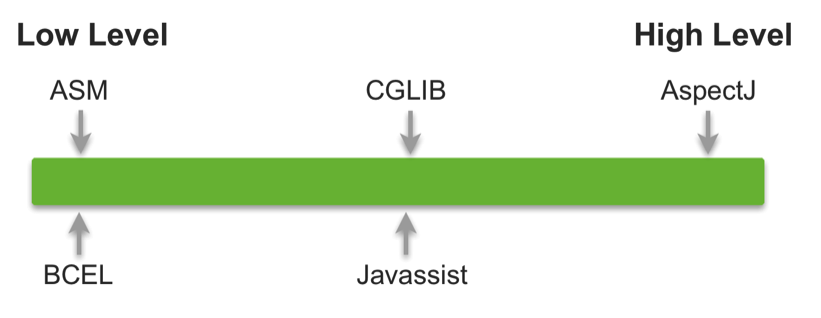
\includegraphics[width=0.8\linewidth]{javassistLevel}
\caption{Bytecode modification levels.}
  \label{fig:bytecodeModificationLevels}
\end{figure}

Unlike many other libraries Javassist offers two levels of API: \textbf{source}-level and \textbf{bytecode}-level (See \figref{bytecodeModificationLevels}\footnote{Figure taken from \href{https://blog.newrelic.com/2014/09/29/diving-bytecode-manipulation-creating-audit-log-asm-javassist/}{blog.newrelic.com}.}\brs{not sure how this figure shows 2 levels of apis}). Using the source-level API, the user can edit a class file without any familiarity with the specifications of the Java bytecode. Knowledge of the Java language is enough since the API is designed only with the vocabulary of Java. On this level the programmer has to write Java source code and Javassist compiles it automatically. The bytecode level allows the user to modify classes by modifying the bytecode directly.

At this point, let us look at a small example\brs{what example?} of how the bytecode manipulation works.

\renewcommand\lstlistingname{Code}
\begin{Java}[caption={Javassist example. This example is taken from the Javassist tutorial.\brs{never mentioned in text}}, label={code:javassistExample}][H]
ClassPool pool = ClassPool.getDefault();
CtClass cc = pool.get("test.Rectangle");
cc.setSuperclass(pool.get("test.Point"));
cc.writeFile();
\end{Java}

\begin{enumerate}
	\item First a \textit{ClassPool} object that controls bytecode modification with Javassist is obtained. With the \textit{ClassPool} a class file (``.class'') can be read on demand for constructing a \textit{CtClass} object.
	
	\item The class \textit{CtClass} (compile-time class) represents the class file meaning that all manipulations are performed on the \textit{CtClass} object. We obtain a reference to the \textit{CtClass} object representing the \code{test.Rectangle} class by invoking the \code{get()} method on the \textit{ClassPool} instance.
	
	\item In this example \chg{the superclass of \code{test.Rectangle} is simply changed to \code{test.Point}}{the only bytecode modification done is changing the superclass of \code{test.Rectangle} to \code{test.Point}}.
	\item Once the bytecode modification is done, the method call \code{writeFile()} on the instance of \textit{CtClass} is necessary to make sure that the changes are reflected on the original class file.
\end{enumerate}
 
\begin{figure}[H]
\centering
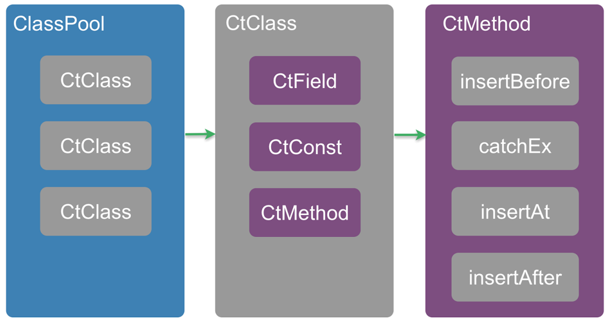
\includegraphics[width=0.8\linewidth]{javassistModules}
\caption{Javassist modules.}
  \label{fig:javassistModules}
\end{figure}

\figref{javassistModules}\footnote{Figure taken from \href{https://blog.newrelic.com/2014/09/29/diving-bytecode-manipulation-creating-audit-log-asm-javassist/}{blog.newrelic.com}.} gives an overview of how the main part of bytecode manipulation with Javassist is built up. The \textit{ClassPool} is simply a container of multiple \textit{CtClasses}. As described before \textit{CtClass} represents class files on which modifications are done. Like typical classes, it can hold compile-time fields, constants or methods. Javassist is capable of adding or modifying classes, behaviors, fields, method invocations, local variables \etc But in our case we mainly address the manipulation of behaviors. It is possible to insert additional source code at the beginning of the method body\chg{ or}{, } at the end or at a specific line. The next example shows how to add code using Javassist.

\begin{Java}[caption={Initial code.}, label={code:initialCode}][H]
public static void main(String[] args) {
	System.out.println("This is an example class.");
}
\end{Java}

\renewcommand\lstlistingname{Bytecode}
\begin{JVMIS}[caption={Initial bytecode.}, label={bytecode:initialBytecode}, breaklines=true][H]
public static void main(java.lang.String[]);
  0: getstatic     #16	// Field java/lang/System.out:Ljava/io/PrintStream;
  3: ldc           #22	// String This is an example class.
  5: invokevirtual #24	// Method java/io/PrintStream.println:(Ljava/lang/String;)V
  8: return
\end{JVMIS}

We want to add one line of code at the beginning of \ins{the main method in} \coderef{initialCode}. \bytecoderef{initialBytecode} is the corresponding bytecode of \coderef{initialCode}.

\renewcommand\lstlistingname{Code}
\begin{Java}[caption={Bytecode modifier.}, label={code:bytecodeModifier}][H]
public class BytecodeModifier {
	public static void main(String[] args) ... {
		ClassPool pool = ClassPool.getDefault();
		CtClass cc = pool.get("insertJavaCodeExample.ExampleClass");

		CtBehavior behavior = cc.getDeclaredMethod("main");
		behavior.insertBefore("System.out.println(\"This is the inserted code.\");");

		cc.writeFile();
		
		//...
	}
}
\end{Java}

With \coderef{bytecodeModifier} we obtain a \textit{CtClass} object \code{cc} at line 5 which represents the class to be modified. At line 7 we get the method we want to modify by adding some source code: \code{System.out.println(``This is the inserted code.'');}. Javassist takes a \textit{java.lang.String} object, compiles it automatically and adds it into the bytecode at the specified location, in our situation at the beginning of the \code{main()} method.

Below \ins{is} the result\chg{,}{\ie} how the \code{main()} method looks like after the modification\brs{this is not really true since the source code was not modified. Say that this main method is equivalent to what we achieved with javastis}. At line 2 we see the inserted code. 

\begin{Java}[caption={Instrumented code: Decompiled with JAD (\secref{jad})}, label={code:instrumentedCodeDecompiled}][H]
public static void main(String args[]) {
	System.out.println("This is the inserted code.");
	System.out.println("This is an example class.");
}
\end{Java}

And of course the \bytecoderef{modifiedBytecode} has changed since Javassist added additional bytecode. The pc-interval [0,3,5] \brs{not a fan on the [] notation, easily confused with references, use something else} represents the added code.

\renewcommand\lstlistingname{Bytecode}
\begin{JVMIS}[caption={Modified bytecode.}, label={bytecode:modifiedBytecode}, breaklines=true][H]
public static void main(java.lang.String[]);
  0: getstatic     #16 	// Field java/lang/System.out:Ljava/io/PrintStream;
  3: ldc           #35	// String This is the inserted code.
  5: invokevirtual #24	// Method java/io/PrintStream.println:(Ljava/lang/String;)V
  8: getstatic     #16	// Field java/lang/System.out:Ljava/io/PrintStream;
 11: ldc           #22	// String This is an example class.
 13: invokevirtual #24	// Method java/io/PrintStream.println:(Ljava/lang/String;)V
 16: return
\end{JVMIS}

%\brs{not sure how the remainder here is relevant, please just give a nice example of some source code, how one would add code to it using javasist and the result} \lt{ganzer paragraph weg?}
%\ugh{Next to these options even a \textit{catch block} can be added. The difference between \code{insertAfter()} and \code{addCatch()} is insertAfter inlines some code right before every return instruction in the method body and addCatch adds a catch clause to the method which handles an exception thrown in the body. So the catch clause is always positioned at the end of the method body. In \figref{insertionCodeExample} below a small insertion example is demonstrated.}

%\begin{figure}[H]
%\centering
%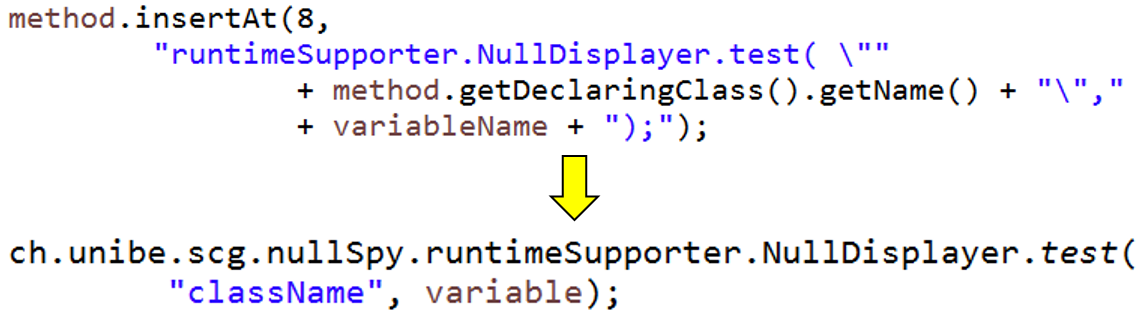
\includegraphics[width=0.9\linewidth]{insertionCodeExample}
%\caption{Inserting code example.}
%  \label{fig:insertionCodeExample}
%\end{figure}

\section{JAD}
\label{sec:jad}
Java Decompier (JAD)\footnote{\url{https://sourceforge.net/projects/jadclipse/}} is a decompiler and \chg{a}{an} Eclipse plugin for the programming language Java. A decompiler is a program that takes an executable file as input, and attempts to create a high level, compatible source file. If the source file is compiled again, it will produce an executable program that behaves the same way as the original one. It is often used in software reverse engineering.

The example \bytecoderef{jad} is decompiled by JAD and the result is the source code right under the example. It is also a good opportunity to present \chg{how}{what} bytecode looks like\brs{looks like -> what, behaves, works, any other action -> how. Also, didn't we have a whole section on bytecode? why is now a good opportunity to present what it looks like? we saw a ton of it 2 sections ago!}.

\begin{JVMIS}[caption={Bytecode example.}, label={bytecode:jad}, breaklines=true]
public void itemStateChanged(java.awt.event.ItemEvent e);
  0  aload_1 [e]
  1  invokevirtual java.awt.event.ItemEvent.getStateChange() : int [23]
  4  iconst_1
  5  if_icmpne 22
  8  aload_0 [this]
  9  getfield org.jhotdraw.applet.DrawApplet$1.this$0 : org.jhotdraw.applet.DrawApplet [12]
 12  aload_1 [e]
 13  invokevirtual java.awt.event.ItemEvent.getItem() : java.lang.Object [29]
 16  checkcast java.lang.String [33]
 19  invokevirtual org.jhotdraw.applet.DrawApplet.loadDrawing(java.lang.String) : void [35]
 22  return
Line numbers:
 [pc: 0, line: 213]
 [pc: 8, line: 214]
 [pc: 22, line: 216]
Local variable table:
 [pc: 0, pc: 23] local: this index: 0 type: new org.jhotdraw.applet.DrawApplet(){}
 [pc: 0, pc: 23] local: e index: 1 type: java.awt.event.ItemEvent
\end{JVMIS}

\renewcommand\lstlistingname{Code}
\begin{Java}[caption={Decompiled bytecode.}, label={code:decompiledBytecode}]
public void itemStateChanged(ItemEvent e) {
	if(e.getStateChange() == 1)
	loadDrawing((String)e.getItem());
}
\end{Java}

JAD is in no way a dependency of NullSpy but it was a big help during the implementation phase\del{.} Since after running NullSpy on a project only the modified bytecode is available. The use of JAD is for the sake of debugging Nullspy; to check whether the modification by Javassist, \ie inserting source code, \chg{has succeeded}{was successful}. Another way to check the result for correctness is looking at bytecode itself but that would have taken a lot more effort and time.

\chapter{NullSpy}
As explained in \charef{introduction}, this project is about providing the user with an additional stack trace containing the information on where the null is assigned to the variable that caused the \npe. \del{In short, the exact location of where a variable was assigned null will be revealed.} \ugh{We will use the term \mr to refer to the variable or object a method is invoked on and that caused the \npe}\brs{Put this where you first time use \mr, here it's completely void of context}.

\chg{Here}{In this chapter} we give a \del{short} overview of how we implementeddel{the core of} NullSpy. We will also address the challenges (\secref{challenges}) we encountered during the implementation as well as the limitations of the tool (\secref{limitations}).

\section{High Level Overview}
\label{sec:highLevelOverview}
The general approach of NullSpy is to statically analyze a project and instrument the bytecode. We can take the three basic steps of NullSpy from \figref{highLevelOverview}: \textit{load, modify, store}. NullSpy is \del{not a GUI but} a console application which takes two parameters. The first argument \ins{to }NullSpy \del{needs} is the path to the \textit{bin}-folder\brs{not all projects neceserally have a bin folder, so you should say something like ``the folder containing the compiled class files '} of the original project and the second one is the destination where the \ugh{developer}\brs{do you mean user?} wants to store the modified project.

\begin{figure}[H]
\centering
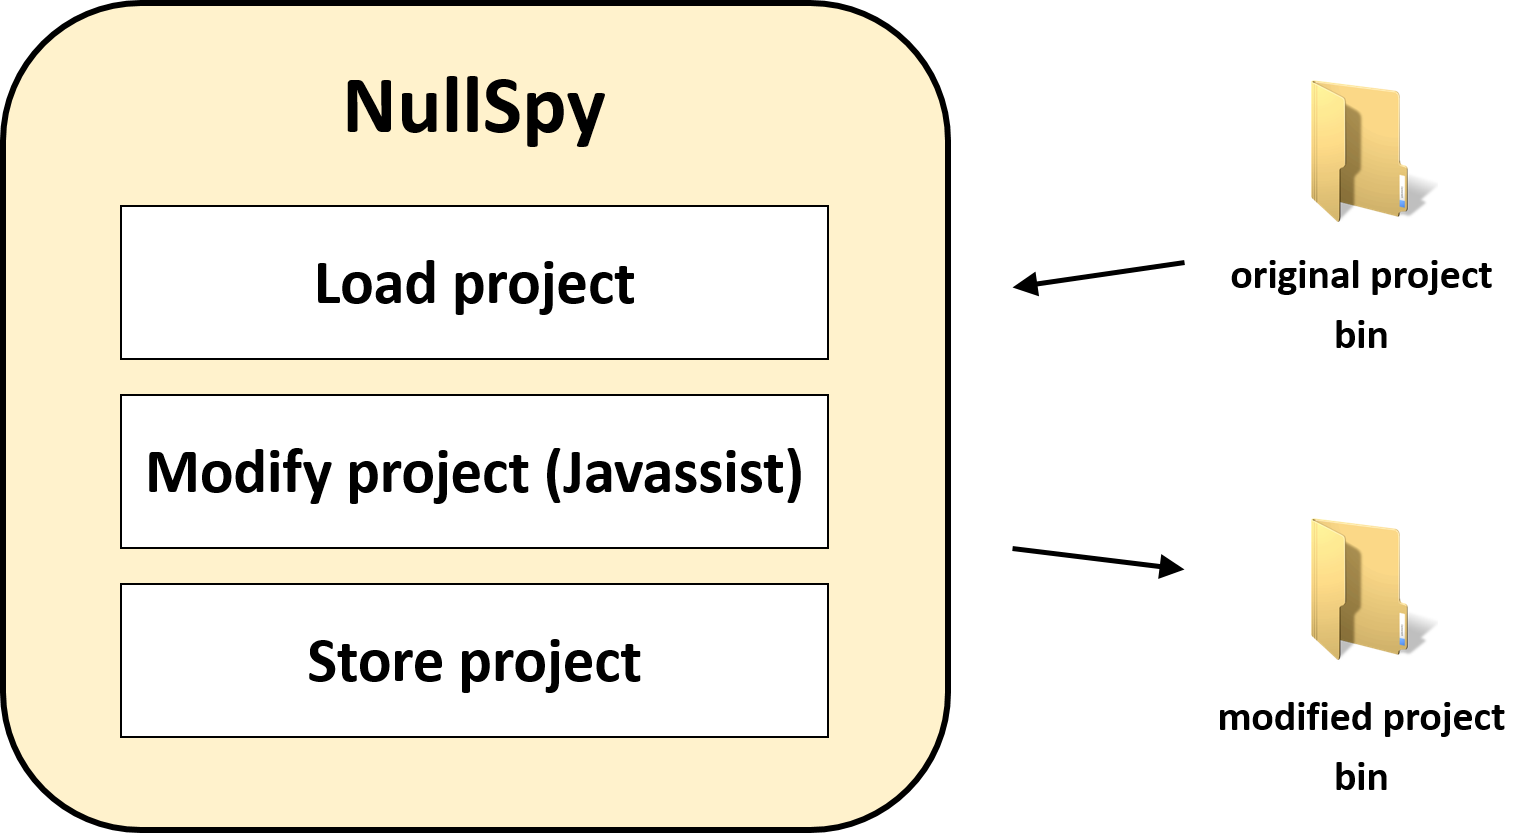
\includegraphics[width=0.8\linewidth]{highLevelOverview3}
\caption{High level overview.}
  \label{fig:highLevelOverview}
\end{figure}

\brs{move here the stuff from the paragraph before about the three steps. You talk abou the 3 steps, then about the console and parameters, then back to the 3 steps, stay on topic}Those three steps of NullSpy are described in \boxref{abstractSteps}\brs{why box? just use enumeration.}:

\begin{figure}[H]
\renewcommand\figurename{List}
	\begin{boxedminipage}{\textwidth}
\begin{enumerate}
\itemsep8pt
	\item Input: Load compiled class files of \ins{the }project \del{we wish for being able to track the null assignments }into NullSpy.
	\item Modification: The modification part \del{contains the }deal\chg{ing}{s} with the bytecode instrumentation and adding modules to the project that \chg{handles}{supports} the inserted code.
	\item Output: Store modified class files to the chosen \ins{output }folder.
   \end{enumerate}
	\end{boxedminipage}
	\caption{NullSpy abstract steps.}
	\label{box:abstractSteps}
\end{figure}

\del{Once the project modification is done it is stored in a destination folder the user has chosen before.} We provide the option to choose the destination is because in case the developer does not want to overwrite the original project with the modified one. This means that the updated bytecode can be stored in another location, keeping the original class files intact. Of course the original project can be replaced by the modified one too. But the developer has to think carefully about it because once replaced, the additional bytecode stays there and the execution time is slightly different than it was before. To get rid of the additional bytecode, the developer has to recompile the source code to get the original class files when needed. This has to be done every time when NullSpy is used on the project.\brs{this belongs where you explain the parameters}

\brs{missing from this section: how is loading done? how is storing done? seems trivial I know, but should be explained. ``Loading is done by traversing all the subfolders of the folder given as a parameter, and extracting all the .class files bla bla bla... Storing is done by recreating the structure from the source folder in the destination folder and storing the modified class files as explained in Subsection 2.2''} 

\section{Low Level Overview}
\label{sec:lowLevelOverview}

\ugh{In this section we will focus on the second abstract step of NullSpy, namely the modification step.}\brs{what does second abstract step mean? just say we focus on the bytecode modification.}  \figref{modificationModules} shows that NullSpy contains three different modules in total. That means each class file of the loaded project will \chg{get in touch}{will be run through} with each of these modules. The first thing we do with the loaded class file is extracting data from its bytecode, then do \chg{some}{the} instrumentation and at the end \chg{adding a}{we add the} run time supporter module to the project.
\brs{the order of the steps in the text does not mach the order in the picture, please update the picture}

\begin{figure}[H]
\centering
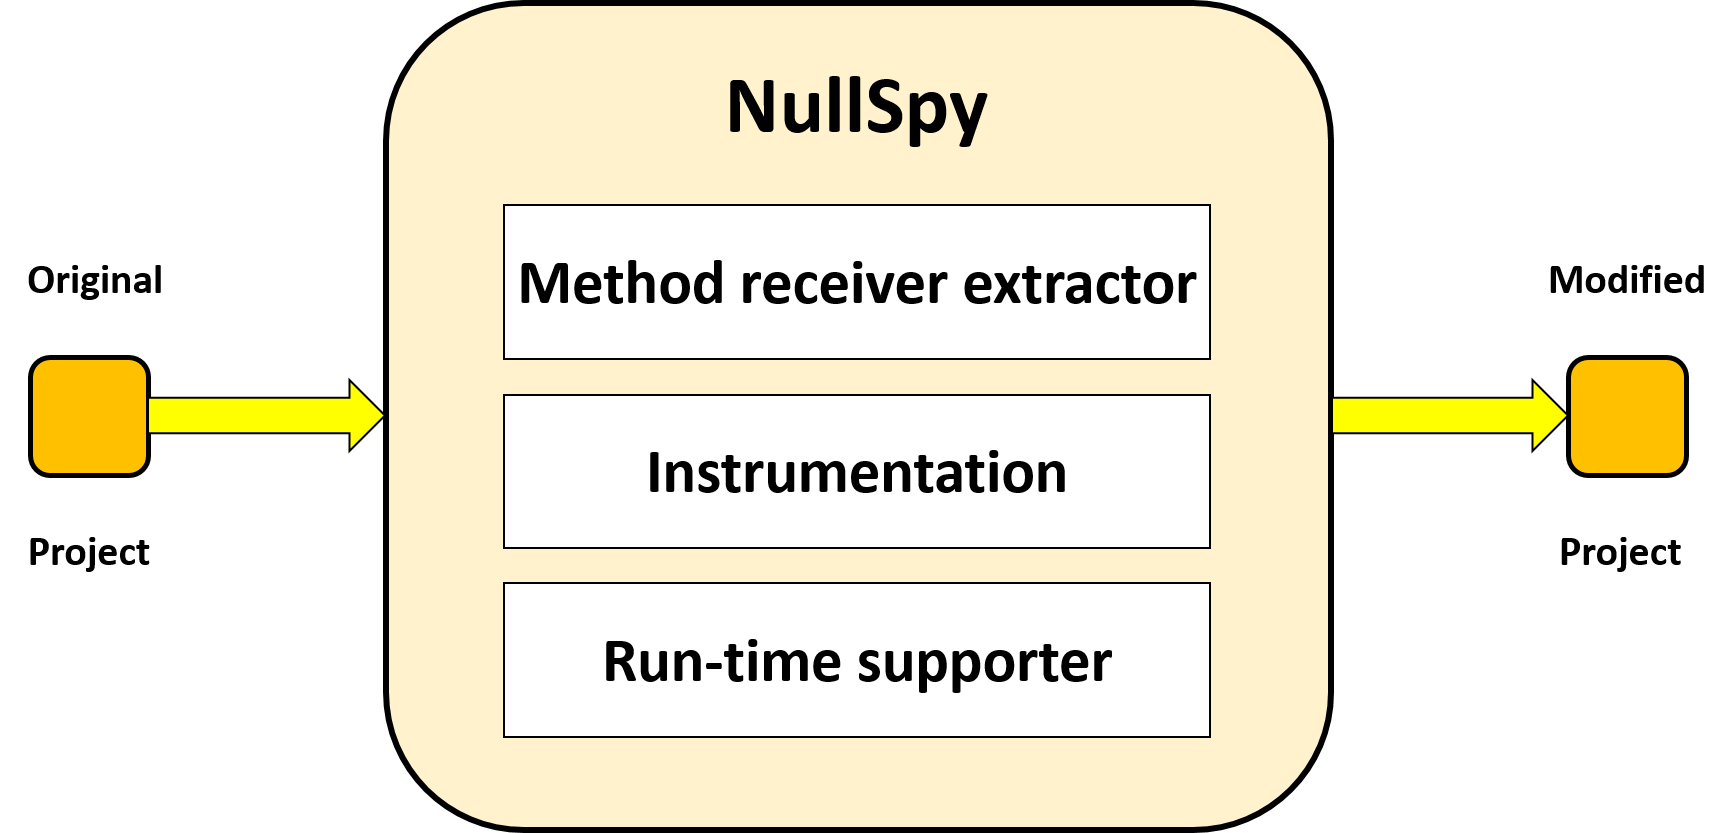
\includegraphics[width=0.8\linewidth]{lowLevelOverview}
\caption{NullSpy modification modules.}
  \label{fig:modificationModules}
\end{figure}

We will look at these modules \ins {in }more detail\del{ed} and explain what \chg{they are all about}{each one does}.

\subsection{\MR Data Collection}
\label{subsec:methodReceiver}
A big part of NullSpy is extracting information from bytecode. One of the item we are interested to get information \chg{from}{about} is the \mr. We use the term \mr to refer to variables on which methods are \chg{performed}{invoked, or whose fields are accessed}.\ugh{ A small example makes is easier to understand: The \mr in code \code{var.method()} is \code{var}}.

We use the \ugh{class}\brs{I'm not sure what you mean by class library... are there method libraries or something?} library Javassist (\secref{javassist}) to extract data from bytecode. Unfortunately, Javassist does not provide the function\ins{ality} to directly get information about the \mr. \chg{What kind of}{The exact} information we need \chg{will be}{is}\brs{will be is future tense and I understand that the reader will read it in the future, but it's already listed now, and if the reader wants to skip ahead she can} listed later in this section. To put it another way, with Javassist we cannot\ins{ directly} extract the \mrs from bytecode. That is why we implemented our own algorithm to get the \mrs. The algorithm contains following steps:

\begin{figure}[H]
\renewcommand\figurename{Algorithm}
	\begin{boxedminipage}{\textwidth}
		\begin{enumerate}
\itemsep8pt
      \item Getting \ins{the }pc-interval of method invocation
      \item Storing all possible \mr interval within the interval of step 1 into an ArrayList
			\item Getting the number of parameters, the method invocation takes
			\item Traversing back the ArrayList the amount of parameters obtained in step 3
			\item Result: \mr interval (pc-interval: see \secref{bytecode})
   \end{enumerate}
	\end{boxedminipage}
	\caption{\Mr algorithm.\brs{very unclear, I have no idea what all this means}}
	\label{alg:methodReceiverAlg}
\end{figure}

A small example how \algref{methodReceiverAlg} is used (code snippet from JHotDraw):

\renewcommand\lstlistingname{Code}
\begin{Java}[caption={Code snippet to demonstrate \algref{methodReceiverAlg}.}, label={code:methodReceiverAlgDemoCode}]
protected void open(final DrawingView newDrawingView) {
	//...
	activePanel.add((Component) getDesktop(), BorderLayout.CENTER);
	//...
}
\end{Java}

We are only looking at line 6\brs{um... the example has only 5 lines of code...} in \coderef{methodReceiverAlgDemoCode}.

\renewcommand\lstlistingname{Bytecode}
\begin{JVMIS}[caption={Bytecode of \coderef{methodReceiverAlgDemoCode}.}, label={bytecode:methodReceiverAlgDemoBytecode}, breaklines=true]
protected void open(org.jhotdraw.framework.DrawingView newDrawingView);
 ...
 144  aload_3 [activePanel]
 145  aload_0 [this]
 146  invokevirtual org.jhotdraw.application.DrawApplication.getDesktop() : org.jhotdraw.contrib.Desktop [271]
 149  checkcast java.awt.Component [274]
 152  ldc_w <String "Center"> [276]
 155  invokevirtual javax.swing.JPanel.add(java.awt.Component, java.lang.Object) : void [254] 
 ...
\end{JVMIS}

\begin{figure}[H]
\renewcommand\figurename{Algorithm}
	\begin{boxedminipage}{\textwidth}
		\begin{enumerate}
			\itemsep8pt
			\item pc-interval: \newline 144-155 (cut everything off what has nothing to do with the method invocation)
			\item ArrayList: \newline [144,[145,149],152]
			\item Number of parameters: \newline 2
			\item Traversing back the amount of parameters: \newline [152] (1) ; [145,149] (2)
			\item Result: \newline 144 = \code{activePanel}
		\end{enumerate}
	\end{boxedminipage}
	\caption{Extract \mr example.\brs{how is this an algorithm?}}
	\label{box:extractMethodReceiverExample}
\end{figure}

In step 1 we had \ugh{big troubles} getting the right interval of the \mr. By only statically analyzing the bytecode it is unapparent where \ins{exactly} the \mr is situated \del{exactly} in bytecode. \del{But} more about the challenges we encountered \ins{can be found }in \subsecref{methodReceiverDifficulties}.

Statically analyzing bytecode for \mr means looking for certain opcodes which matches the regex (Regular expression) \textit{``invoke.*"}. There are exactly five \chg{kinds of}{such} bytecode instruction\ins{s}: \textit{invokedynamic}, \textit{invokeinterface}, \textit{invokespecial}, \textit{invokestatic}, \textit{invokevirtual}. The invocation opcode \textit{invokedynamic} facilitates the dynamic\ins{ly}-typed languages\footnote{Language whose type checking is \del{usually} performed at runtime.} through dynamic method invocation. In our case it can be ignored because NullSpy only supports\ins{ java,} \chg{the}{a} \textit{static\ins{lly}-typed} language\footnote{Language whose type checking is performed at compile time.} \del{Java}.

In case of the \textit{invokestatic} instruction we do not have a \mr \brs{why?}. That is why NullSpy treats it extraordinary \chg{like}{by} ignoring it completely or wrap\ins{ing} it as a \ugh{possible \mr when it is actually a parameter of a method invocation}\brs{this does not make sense to me. if it's a parameter it could be a \mr?}. \chg{In}{For} all other \chg{cases}{invocation bytecodes} we \del{normally }use \chg{the}{our} algorithm to get the \mr. 

\brs{the algorithm is very poorly explained, i still have no idea how you get from pc-interval to any useful information}

After getting the pc-interval of a \mr we gather data about it and store them in an external \textit{csv} file \ugh{due to performance and overhead minimization}\brs{what? why? performance as compared to what?}. The following list \chg{will list}{shows} the information which is stored about the \mr.

\begin{figure}[H]
\renewcommand\figurename{List}
	\begin{boxedminipage}{\textwidth}
		\begin{itemize}
		\itemsep8pt
    \item \ugh{nr}\brs{really? nr?} (\mrs are counted)
		\item lineNumber
		\item variableID (whether it is a local variable or a field)
		\item variableType
		\item isVariableStatic
		\item classWhereVariableIsAccessed
		\item behavior (method)
		\item behaviorSignature
		\item localVariableAttributIndex (if variable is a local variable, else ``empty string'')
		\item fieldDeclaringClassName (if variable is a field, else ``empty string'')
   \end{itemize}
	\end{boxedminipage}
	\caption{\Mr information.}
	\label{box:methodReceiverInfo}
\end{figure}

We will talk about the purpose why these information about the \mr are needed later in this section.

\brs{after reading this subsection I realised it's really hard to follow these details without knowing why we need them. We should have a short overview of the entire process at the beggining of the section, so that the reader has some idea of what's going on and why we need to do this. As it is now, he just has to trust us that this needs to be done, and that's not good.}

\subsection{Variable Data Collection}
\label{subsec:variable}
\ugh{Data about the \mrs plus information about the variables which are assigned an object are needed in NullSpy.} In \ins{the }section before we were looking for instructions which matches the regex \textit{``invoke.*''} for finding \mrs in bytecode. This time we are looking for \chg{following}{the} regexs \textit{``astore.*''} and \textit{``put.*''}. The former refers to local variable assignments and the latter to field assignments. \ugh{After finding one of the assignment NullSpy gathers data about the variable because NullSpy inserts bytecode right after the assignment which represents a method invocation that needs the gained data as parameters. The inserted bytecode represents a test method which tests whether the value assigned to the variable is null and store the gathered information about it}\brs{this is why we need the short overview at the beginning, than we would not need these half baked explanations here and there}. Unlike in getting information about the \mr in \subsecref{methodReceiver} the data about the variables are stored in a HashMap.


In the next two subsections we will look at how those information about the assigned variables are extracted. Due to different variable types and the limitation of Javassist, the way of gathering information about the assignments is performed differently.

\subsubsection{Local Variable}
\label{subsubsec:localVariable}
Unfortunately, Javassist does not provide any support for gaining information about local variables that is why getting the needed data we had to understand how bytecode is constructed. At this point we would like to give a small bytecode introduction.

\begin{figure}[H]
\centering
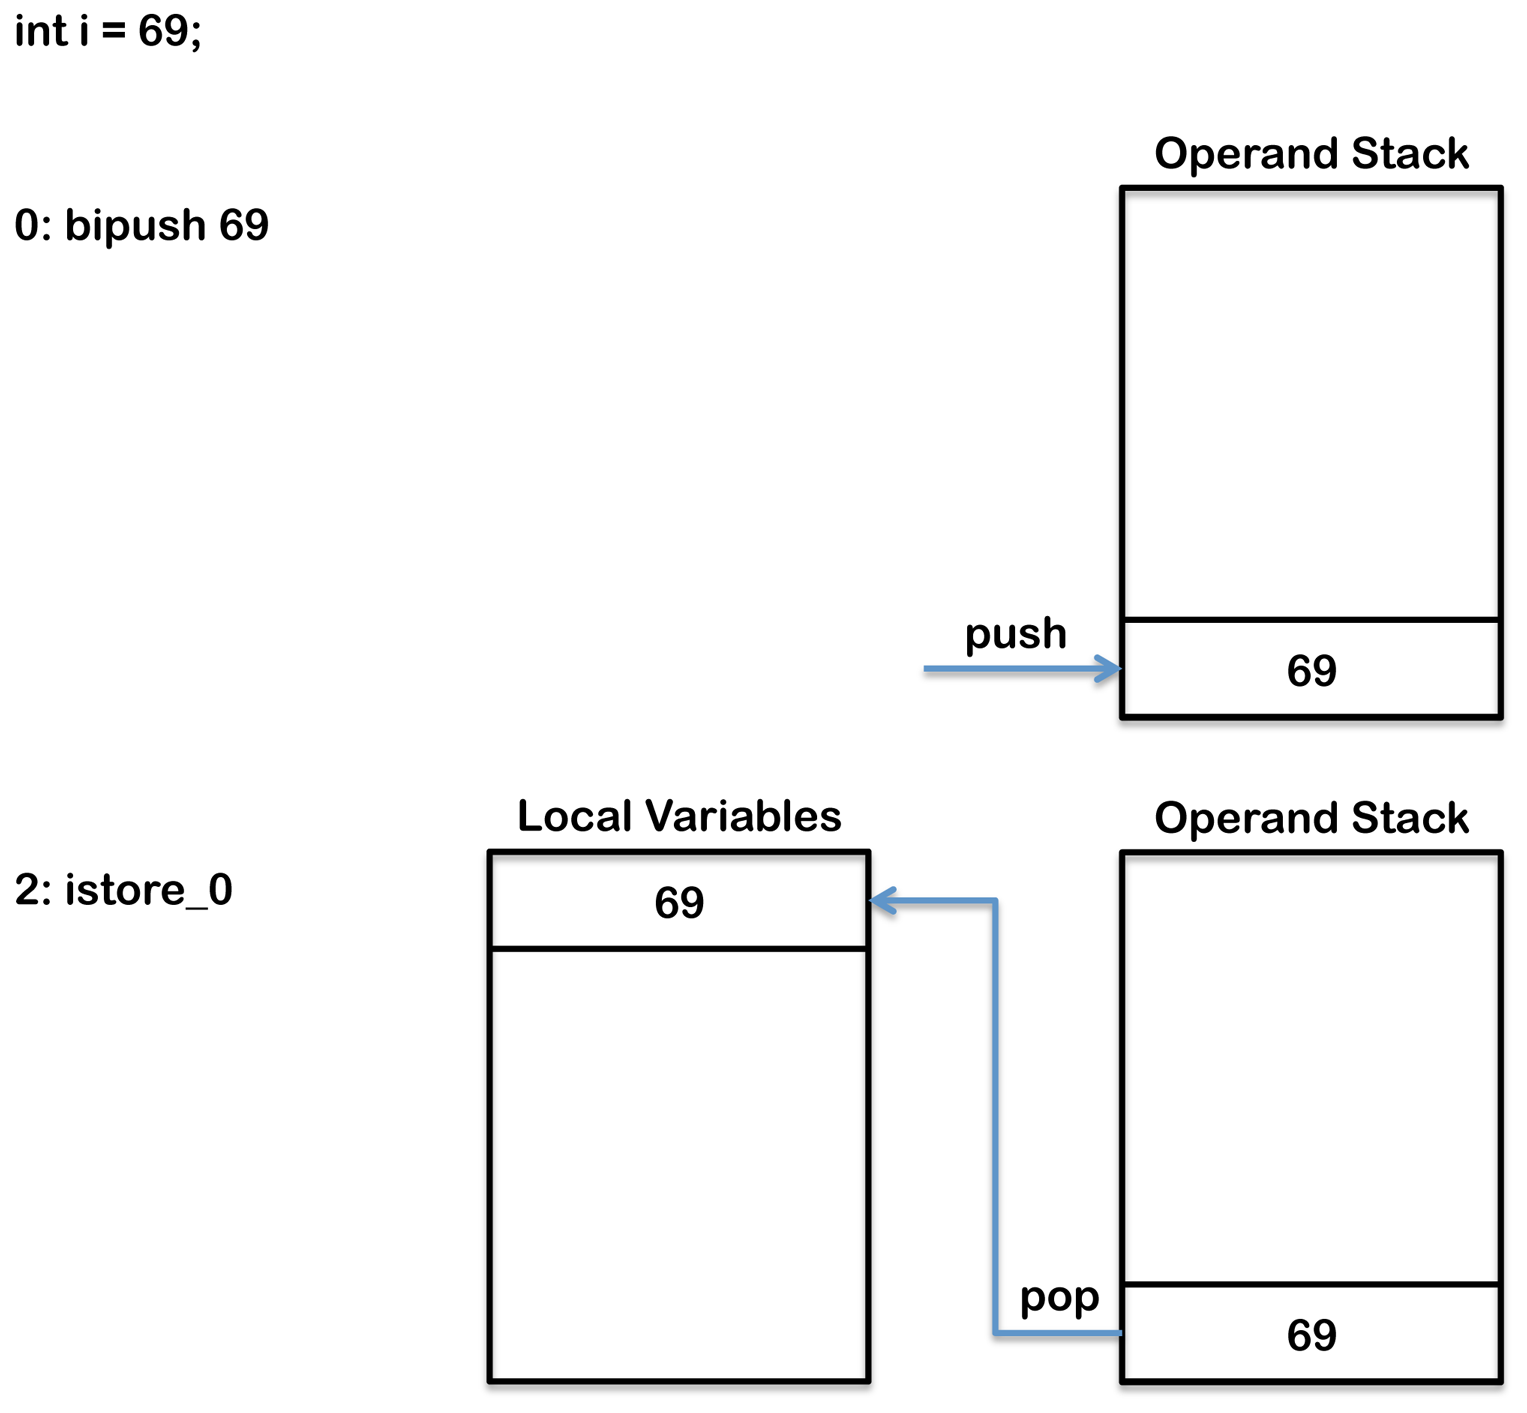
\includegraphics[width=0.8\linewidth]{localVarCreationBytecode}
\caption{Local variable creation\protect.}
  \label{fig:localVarCreationBytecode}
\end{figure}

If a local variable is created, the value assigned to it is pushed onto the operand stack as we can see in \figref{localVarCreationBytecode}\footnote{Figure taken from \href{http://blog.jamesdbloom.com/JavaCodeToByteCode_PartOne.html}{blog.jamesdbloom.com}.}. With the bytecode instruction \textit{``astore.*"} the local variable is popped from the operand stack and stored into a local variable array slot. In which slot it is stored can be extracted from the instruction. Opcodes for storing local variables is composed of one, or in some cases two bytes. There are reserved machine commands for the first four local variables, index-linked from 0 to 3 and each of them contains one byte (astore\_0, astore\_1, astore\_2, astore\_3). If there is no slot number visible in the instruction, it indicates that the slot number is stored in the second byte from where it can be extracted. In addition to storing local variable loading it from the local variable array is possible too, but of course again only with the local variable slot number.

With this short introduction understanding the local variable table should be easier. Each method of a class file contains a local variable table (see \bytecoderef{localVarTable}) with which many information can be read out, \ie the lifespan of a local variable, what it is called, in which slot it is stored and what type it has.

\renewcommand\lstlistingname{Bytecode}
\begin{JVMIS}[caption={Local variable table.}, label={bytecode:localVarTable}, breaklines=true]
Local variable table:
 [pc: 0, pc: 31] local: this index: 0 type: org.jhotdraw.samples.javadraw.JavaDrawApp
 [pc: 0, pc: 31] local: newDrawing index: 1 type: org.jhotdraw.framework.Drawing
 [pc: 5, pc: 31] local: d index: 2 type: java.awt.Dimension
 [pc: 22, pc: 31] local: newDrawingView index: 3 type: org.jhotdraw.framework.DrawingView
\end{JVMIS}

We have to pay attention to get the right local variable every time we bump into one while iterating through bytecode. Every time we hit upon the opcode \textit{``astore.*"} we could only get its slot and the pc where it is situated in the bytecode sequence. In the earlier paragraph the lifespan of the local variable was mentioned. The importance behind this is, as soon as the lifespan of one ends, the slot can be reused by the next instantiated local variable. This way, the local variable table could contain multiple entries with the same local variable slot.

\begin{JVMIS}[numbers=left, caption={Local variable table entries with same slot 2 (line 4\&7).}, label={bytecode:localVarTableDuplicatedSlot}, breaklines=true]
Local variable table:
 [pc: 0, pc: 95] local: this index: 0 type: org.jhotdraw.samples.javadraw.JavaDrawViewer
 [pc: 0, pc: 95] local: filename index: 1 type: java.lang.String
 [pc: 13, pc: 40] local: url index: 2 type: java.net.URL
 [pc: 18, pc: 40] local: stream index: 3 type: java.io.InputStream
 [pc: 28, pc: 40] local: reader index: 4 type: org.jhotdraw.util.StorableInput
 [pc: 44, pc: 94] local: e index: 2 type: java.io.IOException
\end{JVMIS}

After extracting the slot (\ie index: 2) of the local variable we will get the first local variable table entry which contains that slot (\ie line 4). If the pc (\ie pc: 45) of the local variable assignment is not included in the lifespan-pc-interval of the entry (\ie [pc: 13, pc: 40]), the next entry (\ie line 7;  [pc: 44, pc: 94]) with the same slot will be examined until both criteria slot and pc fits. Once those criteria are met we can be positive about having the right local variable table entry to extract the information we need.

\begin{JVMIS}[caption={Line number table.}, label={code:lineNrTable}]
 Line numbers:
  [pc: 0, line: 26]
  [pc: 4, line: 27]
  [pc: 8, line: 29]
  [pc: 16, line: 30]
\end{JVMIS}

Each method of a class file does not only hold a local variable table but also another attribute called line number attribute. This is the mapping table from pc to source code line number. That means after getting the pc of the local variable assignment we can obtain the right line number. The line number is essential for constructing the link which is added to the common exception stack trace.

The other information we need in addition to the line number are: 

\begin{figure}[H]
\renewcommand\figurename{List}
	\begin{boxedminipage}{\textwidth}
\begin{itemize}
		\itemsep8pt
    \item variableID (distinguishes whether the variable is a field or a local variable)
		\item localVariableName
		\item localVariableLineNumber
		\item localVariableType
		\item startPc
		\item storePc
		\item afterPc
		\item className
		\item behavior
		\item localVariableAttributeIndex
		\item localVariableSlot
   \end{itemize}
	\end{boxedminipage}
	\caption{Local variable information.}
	\label{box:localVarInfo}
\end{figure}

\subsubsection{Instance and Class/Static variable (Field)}
\label{subsec:field}
Although Javassist does not support the access to local variable it provides a way for fields. Javassist allows modifying an expression in a method body with the class \code{Javassist.expt.ExprEditor}. In our case we only want to extract some information about the fields instead of any modification, nevertheless this class can be used appropriately. What it does is to scan the bytecodes on instructions like \textit{``putfield"} or \textit{``putstatic"}.

There are only two instructions that indicates an access to a field, but there are actually many different types. To get the meaning of different types see the following list:

\begin{figure}[H]
\renewcommand\figurename{List}
	\begin{boxedminipage}{\textwidth}
		(\textbar\dots\textbar: put value on operand stack for assigning to a field)
\begin{enumerate}
\itemsep8pt
      \item aload\_0, \textbar\dots\textbar, putfield
      \item \textbar\dots\textbar, putstatic
			\item aload.*, \textbar\dots\textbar, putfield
			\item aload\_0, (getfield)+, \textbar\dots\textbar, putfield
			\item getstatic, (getfield)*, \textbar\dots\textbar, putfield
   \end{enumerate}
	\end{boxedminipage}
	\caption{Field keywords.}
	\label{box:fieldKeywords}
\end{figure}
	
Depending on the category the field belongs, different kind of information is stored. For fields 1-2 following information is needed and stored:

\begin{figure}[H]
\renewcommand\figurename{List}
	\begin{boxedminipage}{\textwidth}
\begin{itemize}
		\itemsep8pt
    \item fieldID (which is field or localVar)
		\item fieldname
		\item fieldType
		\item fieldDeclaringClassName (in which class it is instantiated)
		\item isFieldStatic
		\item fieldLineNumber
		\item startPosition (nonstatic: this; static: value loading bytecode for assigning to the field)
		\item storePosistion (putfield/putstatic)
		\item afterStorePosition (right before this pos additional bytecode is inserted)
		\item classWhereFieldIsAccessed (in this case the same as fieldDeclaringClassName)
		\item behavior (method where it is accessed)
		\item indirectVariable (null - explained immediately)
   \end{itemize}
	\end{boxedminipage}
	\caption{Variable information (I).}
	\label{box:variableInfo1}
\end{figure}

In NullSpy we call these fields \textit{``directFields"}. Reading \textit{``direct"} implicates that there must be something like \textit{``indirectFields"}, and that is right. As \textit{``indirectFields"} the fields 3-4 are numbered among. Everything before the instruction \textit{putfield} is termed as \textit{``indirectVariable"}. For those fields more data are needed to store for their identification. Nearly the same as above, except:

\begin{figure}[H]
\renewcommand\figurename{List}
	\begin{boxedminipage}{\textwidth}
\begin{itemize}
\itemsep8pt
      \item classWhereFieldIsAccessed (can be differend than fieldDeclaringClassName)
\item indirectVariable:
\begin{itemize}
\item indirectVariableName
\item indirectVariableType
\item indirectVariableDeclaringClassName
\item isIndirectVariableStatic
\item indirectVariableOpcode (to distinguisch if it is a localVariable or a field)
\end{itemize}
   \end{itemize}
	\end{boxedminipage}
	\caption{Variable information (II).}
	\label{box:variableInfo2}
\end{figure}

With a syntactic example we show how the instructions \textit{``putfield"} and \textit{``putstatic"} are used:

\renewcommand\lstlistingname{Code}
\begin{Java}[caption={Example: \textit{``putfield"} and \textit{``putstatic"}.}, label={code:instrExample}]
public class A {

	private B b = new B();
	private static B b2;

	public void x() {
		
		// |...|: value assigned
		
		// directFields
		this.b = ...; // aload_0, |...|, putfield
		b2 = ...; // |...|, putstatic

		B b3 = new B();
		
		// indirectFields
		b3.c = ...; // aload.*, (getfield)*, |...|, putfield
		b3.c.d = ...
		b.c = ...; // aload_0, (getfield)+, |...|, putfield
		b.c.d = ...;
		b2.c = ...; // getstatic, (getfield)*, |...|, putfield
		b2.c.d = ...;
	}
}

public class B {						
	public C c = new C();																
	...										
}				

public class C {
	public D d = new D();
	...	
}

public class D {
	...
}
\end{Java}

Once the bytecode is modified, the way to get the data of fields needs some adaptation (see \subsecref{variableDifficulties}).

\subsection{Bytecode Adaptation}
\label{bytecodeAdaptation}
Each time encountering a variable assignment we first extract the needed data and directly after this we adapt the class file by adding extra bytecode right after the assignment bytecode to check whether the variable is null or not. If it is null, the information collected before is stored either into the \textit{``localVariableMap"} or into a \textit{``fieldMap"} which are HashMaps.

The added bytecode represents a static method of a class named \code{VariableTester}\footnote{\label{package1}In package \emph{ch.scg.nullSpy.runtimeSupporter}.} which will be added to the modified project after class file modification is done. Depending on the kind of variable analyzed at the moment different bytecode is constructed, meaning different method with different parameter/variable data is added.

There were again some challenges we had to get over, like getting the wanted data after an instrumentation and entering the additional code in the right position of the bytecode sequence (\subsecref{bytecodeAdaptationDifficulties}).

Once we have gone through the bytecode of a Java class, the modified class files are stored in a destination directory as mentioned in \secref{highLevelOverview}. Next to the instrumentation supplementary supporter classes are added to the project. The most important ones are \code{VariableTester}\textsuperscript{\ref{package1}} which tests whether a variable is null or not and \code{NullDisplayer}\textsuperscript{\ref{package1}} which matches data and prints the location of a null assignment when a \npe is thrown.

\section{Challenges}
\label{sec:challenges}
In this section we could like to give present some of the difficulties which occurred during the implementation of NullSpy.

\subsection{Obtaining \MR Data Difficulties}
\label{subsec:methodReceiverDifficulties}
Aforementioned in \subsecref{methodReceiver} (\textit{\MR Data Collection}) we were encountered with a persistent problem, namely getting the pc-interval of the \mr when the interval covers multiple lines in source code. In many development environment the written code can be formatted automatically and as well manually. See following figures:

\begin{Java}[caption={Method invocation split in two lines example.}, label={code:4-1}, firstnumber=31]
Image image = Iconkit.instance().registerAndLoadImage(
	(Component)view, imageName);
\end{Java}

\renewcommand\lstlistingname{Bytecode}
\begin{JVMIS}[caption={Bytecode to \coderef{4-1}.}, label={bytecode:4-2}, breaklines=true]
 0  invokestatic org.jhotdraw.util.Iconkit.instance() : org.jhotdraw.util.Iconkit [22]
 3  aload_1 [view]
 4  checkcast java.awt.Component [28]
 7  aload_0 [this]
 8  getfield org.jhotdraw.samples.minimap.MiniMapDesktop.imageName : java.lang.String [14]
11  invokevirtual org.jhotdraw.util.Iconkit.registerAndLoadImage(java.awt.Component, java.lang.String) : java.awt.Image [30]
14  astore_2 [image]
\end{JVMIS}

\begin{JVMIS}[caption={Line number table/interval to \coderef{4-1}.}, label={bytecode:4-3}, breaklines=true]
[pc: 0, line: 31]
[pc: 3, line: 32]
[pc: 11, line: 31]
\end{JVMIS}


%\begin{figure}[H]
%\centering
%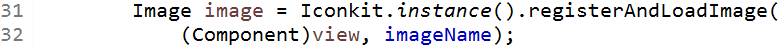
\includegraphics[width=\linewidth]{multipleLine/pic4-1}
%\caption{Method invocation split in two lines example.}
%  \label{fig:pic4-1}
%\end{figure}

%\begin{figure}[H]
%\centering
%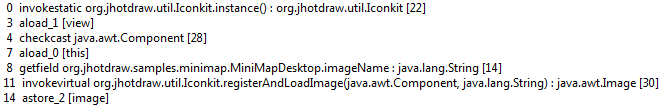
\includegraphics[width=\linewidth]{multipleLine/pic4-2}
%\caption{Bytecode to \figref{pic4-1}.}
%  \label{fig:pic4-2}
%\end{figure}

%\begin{figure}[H]
%\centering
%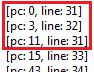
\includegraphics[width=0.3\linewidth]{multipleLine/pic4-3}
%\caption{Line number table/interval to \figref{pic4-1}.}
%  \label{fig:pic4-3}
%\end{figure}

Figure shows a normal method invocation which is split into two lines in source code. This cannot be figured out by just looking at the bytecode therefore the line number attribute (\coderef{lineNrTable}) has to be consulted too. There is no \mr in the figure because the \mr would contain a method invocation itself, what is not supported in NullSpy. Another \mrs NullSpy does not support are elements of collections due to its complex structures that can be stored in the collections.

Only looking at bytecode is not enough, so we are looking at the line number attribute. Line number \textit{31} (\bytecoderef{4-3}) is listed twice, this indicates that the method invocation is split into multiple line in source code. The former declares the starting point of the interval and the latter the end of it. How to get the pc-interval will be presented shortly. But first take a look at more examples:

\renewcommand\lstlistingname{Code}
\begin{Java}[caption={Alternating line number example.}, label={code:3-1}, firstnumber=127]
Connector oldConnector = ((ChangeConnectionHandle.UndoActivity)
			getUndoActivity()).getOldConnector();
\end{Java}

\renewcommand\lstlistingname{Bytecode}
\begin{JVMIS}[caption={Bytecode to \coderef{3-1}.}, label={code:3-2}, breaklines=true]
47  aload_0 [this]
48  invokevirtual org.jhotdraw.standard.ChangeConnectionHandle.getUndoActivity() : org.jhotdraw.util.Undoable [72]
51  checkcast org.jhotdraw.standard.ChangeConnectionHandle$UndoActivity [76]
54  invokevirtual org.jhotdraw.standard.ChangeConnectionHandle$UndoActivity.getOldConnector() : org.jhotdraw.framework.Connector [142]
57  astore 7 [oldConnector]
\end{JVMIS}

\begin{JVMIS}[caption={Line number table/interval to \coderef{3-1}.}, label={code:3-3}, breaklines=true]
[pc: 47, line: 128]
[pc: 51, line: 127]
[pc: 54, line: 128]
[pc: 57, line: 127]
\end{JVMIS}

%\begin{figure}[H]
%\centering
%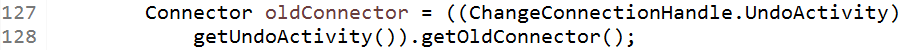
\includegraphics[width=\linewidth]{multipleLine/pic3-1}
%\caption{Alternating line number example.}
%  \label{fig:pic3-1}
%\end{figure}

%\begin{figure}[H]
%\centering
%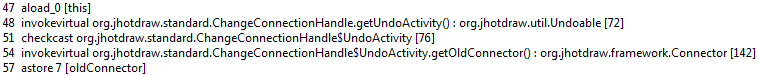
\includegraphics[width=\linewidth]{multipleLine/pic3-2}
%\caption{Bytecode to \figref{pic3-1}.}
%  \label{fig:pic3-2}
%\end{figure}

%\begin{figure}[H]
%\centering
%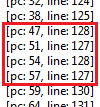
\includegraphics[width=0.3\linewidth]{multipleLine/pic3-3}
%\caption{Line number table/interval \figref{pic3-1}.}
%  \label{fig:pic3-3}
%\end{figure}

Special about this example is that the multiple line interval does not start with the smaller line number and end with the bigger one, apart from that it is alternated stored in the line number attribute.

\renewcommand\lstlistingname{Code}
\begin{Java}[caption={Nested interval example.}, label={code:2-1}, firstnumber=149]
for (int i = 0; i < ColorMap.size(); i++)
	choice.addItem(
		new ChangeAttributeCommand(
			ColorMap.name(i),
			attribute,
			ColorMap.color(i),
			this
		)
	);
\end{Java}

\renewcommand\lstlistingname{Bytecode}
\begin{JVMIS}[caption={Bytecode to \coderef{2-1}.}, label={code:2-2}, breaklines=true]
 8  iconst_0
 9  istore_3 [i]
10  goto 37
13  aload_2 [choice]
14  new org.jhotdraw.standard.ChangeAttributeCommand [213]
17  dup
18  iload_3 [i]
19  invokestatic org.jhotdraw.util.ColorMap.name(int) : java.lang.String [246]
22  aload_1 [attribute]
23  iload_3 [i]
24  invokestatic org.jhotdraw.util.ColorMap.color(int) : java.awt.Color [252]
27  aload_0 [this]
28  invokespecial org.jhotdraw.standard.ChangeAttributeCommand(java.lang.String, org.jhotdraw.framework.FigureAttributeConstant, java.lang.Object, org.jhotdraw.framework.DrawingEditor) [222]
31  invokevirtual org.jhotdraw.util.CommandChoice.addItem(org.jhotdraw.util.Command) : void [225]
34  iinc 3 1 [i]
37  iload_3 [i]
38  invokestatic org.jhotdraw.util.ColorMap.size() : int [256]
41  if_icmplt 13
\end{JVMIS}

\begin{JVMIS}[caption={Line number table/interval to \coderef{2-1}.}, label={code:2-3}, breaklines=true]
[pc: 8, line: 149]
[pc: 13, line: 150]
[pc: 14, line: 151]
[pc: 18, line: 152]
[pc: 22, line: 153]
[pc: 23, line: 154]
[pc: 27, line: 155]
[pc: 28, line: 151]
[pc: 31, line: 150]
[pc: 34, line: 149]
\end{JVMIS}

%\begin{figure}[H]
%\centering
%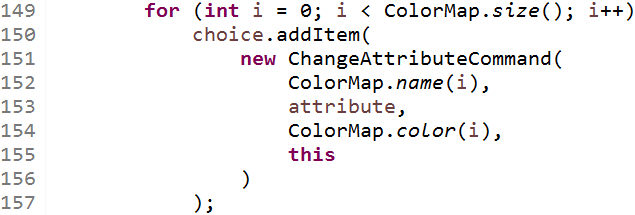
\includegraphics[width=\linewidth]{multipleLine/pic2-1}
%\caption{Nested interval example.}
%  \label{fig:pic2-1}
%\end{figure}

%\begin{figure}[H]
%\centering
%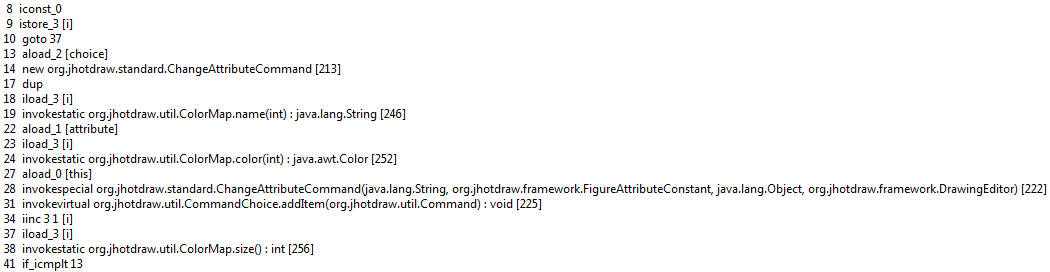
\includegraphics[width=\linewidth]{multipleLine/pic2-2}
%\caption{Bytecode to \figref{pic2-1}.}
%  \label{fig:pic2-2}
%\end{figure}

%\begin{figure}[H]
%\centering
%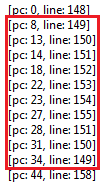
\includegraphics[width=0.3\linewidth]{multipleLine/pic2-3}
%\caption{Line number table/interval to \figref{pic2-1}.}
%  \label{fig:pic2-3}
%\end{figure}

Neither in bytecode nor in line number attribute we can extract the exact interval of method invocations. Generally, we cannot distinguish if the interval represents a method invocation or a loop. Another interesting thing is that in the figure multiple corresponding pcs are included.
\lt{change to scntactic example}
\renewcommand\lstlistingname{Code}
\begin{Java}[caption={Incomplete interval example.}, label={code:5-1}, firstnumber=22]
fooTestSupporter
	.bla(getObject(),
		staticMethod(o),
		fooTestSupporter2.bla2(null,
			o));
\end{Java}

\renewcommand\lstlistingname{Bytecode}
\begin{JVMIS}[caption={Bytecode to \coderef{5-1}.}, label={code:5-2}, breaklines=true]
18  aload_1 [fooTestSupporter]
19  invokestatic isFieldOrLocalVariableNullExample.testMethodCall.FooTest.getObject() : java.lang.Object [26]
22  aload_3 [o]
23  invokestatic isFieldOrLocalVariableNullExample.testMethodCall.FooTest.staticMethod(java.lang.Object) : java.lang.Object [30]
26  aload_2 [fooTestSupporter2]
27  aconst_null
28  aload_3 [o]
29  invokevirtual isFieldOrLocalVariableNullExample.testMethodCall.FooTestSupporter.bla2(java.lang.Object, java.lang.Object) : java.lang.Object [34]
32  invokevirtual isFieldOrLocalVariableNullExample.testMethodCall.FooTestSupporter.bla(java.lang.Object, java.lang.Object, java.lang.Object) : void [38]
\end{JVMIS}

\begin{JVMIS}[caption={Line number table/interval to \coderef{5-1}.}, label={code:5-3}, breaklines=true]
[pc: 18, line: 22]
[pc: 19, line: 23]
[pc: 22, line: 24]
[pc: 26, line: 25]
[pc: 28, line: 26]
[pc: 29, line: 25]
[pc: 32, line: 23]
\end{JVMIS}


%\begin{figure}[H]
%\centering
%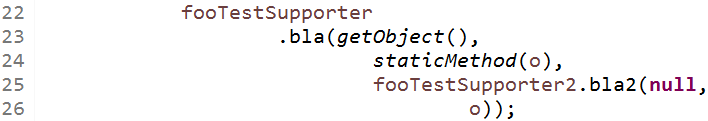
\includegraphics[width=\linewidth]{multipleLine/pic5-1}
%\caption{Incomplete interval example.}
%  \label{fig:pic5-1}
%\end{figure}

%\begin{figure}[H]
%\centering
%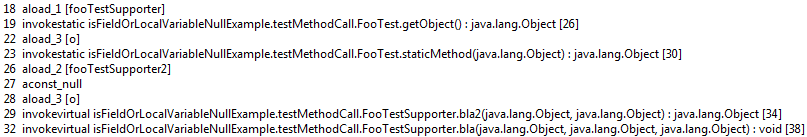
\includegraphics[width=\linewidth]{multipleLine/pic5-2}
%\caption{Bytecode to \figref{pic5-1}.}
%  \label{fig:pic5-2}
%\end{figure}

%\begin{figure}[H]
%\centering
%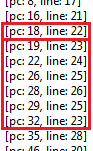
\includegraphics[width=0.3\linewidth]{multipleLine/pic5-3}
%\caption{Line number table/interval to \figref{pic5-1}.}
%  \label{fig:pic5-3}
%\end{figure}

By using the algorithm we only get the interval from pc 19-32, but actually pc 18 also belongs to the interval. That the missing pc is missing will be detected in step 4\&5 when traversing back the ArrayList by the number of parameters. If it is not a static method invocation and there is not enough possible \mrs stored in that ArrayList to traverse back, the missing pc is added in retrospect.

\renewcommand\lstlistingname{Pseudocode}
\begin{Java}[caption={Multiple line interval algorithm.}, label={alg:multipleLineAlg}]
i = index in line number attribute which contains the invoke.* opcode

if (lineNrAttribute[j>i] <= lineNrAttribute[i]) {	
			
	if (isAlternating(i,j))
		return getAlternatingInterval(i, j);
		
	// non-alternating
	b = j which has the smallest line number after j;
	a = corresponding index to b; // index<k which has the same line number as b||k
	return getNonAlternatingInterval(a, b);	
	
} else if (lineNrAttribute[j<i] == lineNrAttribute[i]) {

		b = i;
		a = j;
		return getInterval(a, b);
		
}	
\end{Java}

This pseudocode will give a very rough idea how the invocation interval can be read out. The detailed implementation can be seen in the classes \code{MultipleLineManager}\footnote{\label{package2}In package \emph{ch.unibe.scg.nullSpy.instrumentator.controller.methodInvocation}.} and \code{MethodInvocationAnalyzer}\textsuperscript{\ref{package2}}.

\subsection{Obtaining Variable Data Difficulties - Fields}
\label{subsec:variableDifficulties}
We previously mentioned that NullSpy first collects data about fields and we met some difficulties regarding this. By using the method \code{loopBody()} from class \code{Javassist.expt.ExprEditor} (\subsecref{field}) for gathering information caused those troubles because it loops through the GIVEN \code{methodInfo} which contains the bytecode sequence of a method. Even after finding a field assignment and adding some additional bytecode to it, the method still iterates through the unchanged \code{methodInfo} it got as parameter without the additional bytecode. Getting the right start-pc of a field assignment is not a straight forward process as it may seem.

After entered extra instructions the method \code{loopBody()} iterates onwards until it finds a key which indicates an access to a field. Normally, Javassist provides a method with which the start-pc of the field access can be find out easily, but in our case not due to bytecode alternation. This method returns the start-pc of the field as if there was no changes, however it actually has to return a bigger start-pc than it does. The start-pc is needed to distinguish in what category the field has to be assigned to (\subsecref{field}).

To find the right start-pc of the field assignment, we compare the start-pc returned by a method of Javassist with the \code{afterStorePc} of the previously found field assignment. Every time an assignment is found we store it as a reference for the next assignment to obtain the right data. Even for the store-pc of an assignment (\textit{``put.*"} the last found field is essential. If there is more interest how those pcs are obtained, please see the class \code{FieldAnalyzer}\footnote{In package \emph{ch.unibe.scg.nullSpy.instrumentator.controller}.}.

\subsection{Bytecode Adaptation Difficulties}
\label{subsec:bytecodeAdaptationDifficulties}
The reason why we decided to use Javassist for our NullSpy project is because the thought of only using the source-level API \figref{bytecodeModificationLevels} to implement everything. It would have been much easier to only operate at source-level instead of learning how to read bytecode or extract data from it or enter extra code into it, yet at the end we still had to do everything at bytecode-level.

One big problem encountered while inserting the test method between an assignment and a closing bracket \code{\}}. We tried to insert additional code as shown in \figref{insertionCodeExample} by specifying the exact line number where it should be entered in source code. Unfortunately Javassist first checks the specified line whether it contains some code (only symbols excluded). If there is no code at that line it computes the next line that contains some and inserts the test method right before it. Please visualize a situation where for example a local variable is created/instantiated at the end of a \code{if-body}. In this situation Javassist adds the extra code right before the next code line which is outside the existing scope of the local variable.

\renewcommand\lstlistingname{Code}
\begin{Java}[caption={Bytecode adaptation example.}, label={code:bytecodeAdaptationExample_1}]
Object fontName;
if (fName.startsWith("A")) {
	fontName = new Arial();
} else {
	fontName = new Calibri();
}
\end{Java}

\begin{Java}[caption={Wrong Adaptation to \coderef{bytecodeAdaptationExample_1}.}, label={code:bytecodeAdaptionExample_2}]
Object fontName;
if (fName.startsWith("A")) {
	fontName = new Arial();
 } else {
	--<inserted code which takes ``fontName'' as parameter>--
	fontName = new Calibri();
}
\end{Java}


That is why changed the way to insert the test method at bytecode-level. Like this we first have to build up the bytecode sequence and then enter it before a specific pc. Please take a look at the class \code{ByteCodeAdapter}\footnote{In package \emph{ch.unibe.scg.nullSpy.instrumentator.controller}.} how the bytecode sequence is created.

There are of course many other small problems during the implementation of NullSpy but these mentioned are the most troublesome ones.

\section{Limitations}
\label{sec:limitations}
During the implementation of NullSpy we had to change the concept few times due to limitations or an overhead that could have grown immense.

Our first idea of how NullSpy could track the \npes is to gather information about variable assignment, which is the case now, and also inject another test method right before each method invocations. In small projects this way could have worked fine but in larger projects which could contain hundreds of classes with a lot of method invocations the execution time would be strongly influenced.

Being able to collect data about variables we still are not able to avoid injecting bytecode even it affects the runtime. Related to this issue a limitation about Javassist is mentioned before namely inserting bytecode right before a closing bracket (\subsecref{bytecodeAdaptationDifficulties}). Because of this it highly depends on the location where additional code should be inserted whether using the source-level API is possible or not. \ugh{Avoiding checking all the location where something new should be added it is more secure to do this on bytecode-level.}\lt{ändern} But in cases like entering something at the beginning or at the end of a method body the source-level is just fine.

Another limitation of Javassist to mention is that it does not provide anything to get information about \mrs. It only allows one to extract information about local variables, fields and method invocations itself. The programming language Java also does not provide any information about the \mr, since the exception object or the stack trace element only contains the class, file, method name and the line number. Nonetheless making possible to gather data about them the algorithm discussed before (see \algref{methodReceiverAlg}) fulfills the missing task.

The last limitation we want to discuss here is that unfortunately NullSpy is not capable to track the root of \npes that are originated in a null which was returned of a method call or in an element of a collection. Why those situations are not supported in NullSpy is because of the impossibility way to store them, e.g. imagine a nested ArrayList or a HashMap and a never ending return value of method invocations. So we lack something tangible to compare with each other, get a hit and read the location out of the hit (\secref{futureWork}).

\chapter{Validation}
\label{ch:validation}
This chapter will provide some numbers to compare the execution time each project takes, the original and the instrumented one. To get the numbers we instrumented the example project JHotDraw. 

\section{JHotDraw}
\label{sec:jhotdraw}
{JHotDraw\footnote{\protect\url{http://www.jhotdraw.org/}}} also served to check whether the logic of the bytecode manipulation behind NullSpy is working as desired. JHotDraw is an open-source Java GUI framework for technical and structured Graphics. It is big enough to get reliable numbers and it provides many different cases we had to take care of in NullSpy. Also thanks to Nevena Milojkovi\'{c} and her experience with the combination Javassist and JHotDraw we as well decided to test NullSpy on it.

\section{Execution Time Difference}
\label{sec:execTimeDiff}
How did we get the numbers? First of all, of course another executable jar file of the modified project has to be created. The steps to it are followings: load project, modify project, store modified project, build project that creates an executable jar file of the original project and one of the modified one. We then simulate the terminal with a Java class to run each jar thirty times and calculate the average. The next table lists each execution time and the average:

\begin{table}[H]
\centering
\begin{tabular}{ l | S[table-format=1.3] | S[table-format=1.3]|}
\cline{2-3}	  &\textbf{Original project} & \textbf{Modified project}\\ \cline{2-3}
	1	& 7.223	& 7.442	\\ \cline{2-3}
	2	& 7.427	& 7.738	\\ \cline{2-3}
	3	& 7.171	& 7.893	\\ \cline{2-3}
	4	& 7.035	& 7.379	\\ \cline{2-3}
	5	& 7.488	& 7.458	\\ \cline{2-3}
	6	& 7.194	& 7.691	\\ \cline{2-3}
	7	& 6.849	& 7.472	\\ \cline{2-3}
	8	& 7.286	& 8.068	\\ \cline{2-3}
	9	& 7.083	& 7.519	\\ \cline{2-3}
	10 & 7.27	& 7.55	\\ \cline{2-3}
	11 & 7.16	& 7.177 \\ \cline{2-3}
	12 & 7.161  & 7.55	\\ \cline{2-3}
	13 & 7.225	& 7.223	\\ \cline{2-3}
	14 & 7.037	& 7.316	\\ \cline{2-3}
	15 & 7.067	& 7.54	\\ \cline{2-3}
	16 & 6.975	& 7.77	\\ \cline{2-3}
	17 & 7.287	& 7.117	\\ \cline{2-3}
	18 & 7.52	  & 7.488	\\ \cline{2-3}
	19 & 7.303	& 7.35	\\ \cline{2-3}
	20 & 6.942	& 7.307	\\ \cline{2-3}
	21 & 7.147	& 7.535	\\ \cline{2-3}
	22 & 7.222	& 7.644	\\ \cline{2-3}
	23 & 7.145	& 7.32	\\ \cline{2-3}
	24 & 7.334	& 8.187	\\ \cline{2-3}
	25 & 7.364	&7.488	\\ \cline{2-3}
	26 & 7.269	&7.942	\\ \cline{2-3}
	27 & 7.441	&7.943	\\ \cline{2-3}
	28 & 7.223	&7.467	\\ \cline{2-3}
	29 & 6.912	&7.647	\\ \cline{2-3}
	30 & 7.363	&7.784	\\ \cline{2-3}
	\cline{2-3}
	\end{tabular}
	\caption{Execution time.}
	\label{tab:executionTime}
\end{table}

\begin{table}[H]
	\centering
	\begin{tabular}{ | S[table-format=1.4] | S[table-format=1.6] |}
		\hline	
		\textbf{Original project} & \textbf{Modified project}\\ \hline
		7.2041	&	7.566834 \\
		\hline
	\end{tabular}
	\caption{Average time.}
	\label{tab:averageTime}
\end{table}

The runtime of the modified project takes 0.362734s longer than the original one, this means after adding additional code to the project results in approximately \textbf{5\%} overhead. This small overhead is quite negligible. But this numbers have to be interpreted with caution because the overhead is only measured on JHotDraw.

\chapter {Conclusion and Future Work}
\label{ch:conclusionFutureWork}
Now we have come so far to retrospect (step back and have a critical loot at) the entire project for summarizing what goals we have achieved so far and for proposing further aims that could be completed in the future. In a small section we also want to talk about the gained experience during the whole project.

\section{NullSpy}
\label{sec:nullSpy}
Happily, we could say here that we successfully managed to meet the main purpose we have set at the beginning of the project. NullSpy is now capable to tracking the \npes to its root and provide the user with more information about its origin without spending much time on finding it. The most important steps which lead to the success of NullSpy are listed below:

\begin{enumerate}
\item Extract and gather information about all \mrs because method invocations on these causes \npes. To achieve this, we developed an algorithm (\algref{methodReceiverAlg}) with the function of finding \mrs and extracting data from it by only doing static bytecode analysis. The information about it is then stored as an external csv file. It is needed for a comparison in in a later step.

\item Again collecting data, but this time about variable assignments namely local variables and fields. Here next to the static bytecode analysis additional instructions are inserted to the class files to check right after the assignment if the variable is assigned to the special value \code{null}. If this is the case everything about the variable is stored in a HashMap which serves for a comparison too. It is stored in a HashMap because if a variable is assigned to another object than null, it will be deleted from the HashMap.

\item NullSpy does only handle the uncaught \npe which means we can wrap up the main method with a catch block. In this catch block the class name and the line number where the \npe occurred is extracted from the stack trace. This information is passed to a method in which the parameter helps to find the guilty \mr. With the hit the exact location where that variable was set to null can be derived from the HashMap.

\item All the additional needed classes are added to the project after it is modified and stored in a folder the user has chosen. Being able to run the modified project of course a jar file is created. In our case JHotDraw already provides a \textit{build.xml} which we had to alternate a little bit.
\end{enumerate}

During the implementation we were encountered with many difficulties. Some of those we were able to solve and some not unfortunately. Those unsolved ones could be proposed as goals of future work. The next section will list some of them.

\section{Future Work}
\label{sec:futureWork}
\subsection{Support unsupported \mrs and variable assignments}
As mentioned in (\secref{limitations}), if the cause of a \npe lies in an element of a collection or in an object that is returned by a method invocation, it cannot be tracked to its assignment location. Come up with a way to extract and store information could be a future aim. Of course gathering information about the \mrs has to be improved too.

\subsection{Track \npe root for all projects}
As now our goal in this project was tracking null assignments of JHotDraw. First of all, we had to make sure that building JHotDraw works properly with the additional classes. To fulfil this task manual changes on the build.xml was necessary. If this can be done automatically by NullSpy it would be much better.

Next to this we only looked at the assignment and \mr types which appear in JHotDraw itself. There could be other types that are not covered in NullSpy depending on projects. In case NullSpy is used on projects that contain not supported issues improving it to cover them can be added to the toDo list.

\subsection{Plug-in for Eclipse}
Last target for future work to mention here is transform NullSpy into an Eclipse compatible plug-in project. After integrated it with Eclipse the null tracking can be started without any expenses on how to manipulate the build.xml if there is one or even bother to create an executable jar file out of it.

For now, we can only think of these future work that could improve NullSpy to give it more value.

\section{Personal Experience}
At the beginning, after reading the description of the project I had no clue how to approach its goal at all. Since this is my first big project on my own but with help from two experienced research assistants I learned a lot, especially in the matter of programming.

As the project is all about manipulating class files, here with Javassist, we first had to learn how bytecode is constructed and get familiar with Javassist. Luckily there is a very good tutorial that teaches one how to use it. This class library however does not cover everything we needed. Thanks to this we had to deal with the lack extensively and learned quite a lot about working on bytecode-level.

Next to getting familiar with bytecode we also had to invent algorithms like that of extracting \mrs from the bytecode or that of getting the pc-interval of a \mr. It was quite interesting to invent those as these are the first ones that fulfill more complex tasks.

Debugging: It is not as easy as it seems. Sometimes it took hours to find the cause of a small bug, and after fixing it another occurs. The reason why it took that long to debug is because along with checking whether the logic of our code was right we also had to find the right bytecode position to ensure the implementation does what it is created for.

Coding beautifully the way so that it will not smell was another challenge due to lack of experience. Sometimes I tended to put everything in one class instead of abiding by the single responsibility principle. Therefore, refactoring the whole project multiple times was necessarily which also took some time. Best before starting to code is to clearly thinking through what is needed, how the structure should look like and what kind of responsibility each class of the project should take for gaining time for other things.

We also came in contact with the building XML file and the jar file. Concerning the XML file, we gained experience by learning a new language by modifying it that it also creates a jar file out of the modified project. 

\chapter {Anleitung zu wissenschaftlichen Arbeiten}
NullSpy is a program which helps Java developers to find the root of \npes by providing an additional link next to the common stack trace. The key idea behind NullSpy is to help developers to save time fixing bugs which are caused by \npe. Of course this approach tries to provide this service by keeping the overhead to a minimum. To demonstrate how NullSpy works, this chapter serves as a small tutorial that takes JHotDraw as the testing project to show the feature of NullSpy.

\section{Installation}
\label{sec:installation}
For this tutorial JHotDraw is needed. In order to download it, visit the following site and download ``JHotDraw6.0 beta 1" (version we worked with during the implementation of NullSpy):\\
\href{http://www.jhotdraw.org}{www.jhotdraw.org}\\
Unpack the archive and store it to a location of your choice. To be able to run JHotDraw additional libraries are used, that are not included in JHotDraw itself. Following libraries are to be downloaded:\\
``batik-all-1.7": \href{http://www.java2s.com/Code/Jar/b/Downloadbatikall17jar.htm}{www.java2s.com/Code/Jar/b/Downloadbatikall17jar}\\
``jdo": \href{http://www.java2s.com/Code/Jar/j/Downloadjdojar.htm}{www.java2s.com/Code/Jar/j/Downloadjdojar}\\
Again unpack those archives and store them in a lib folder in your JHodDraw project.

Running the tests of JHotdraw with the commando line the location of libraries ``hamcrest" and ``junit" are needed, which are normally also downloaded when the programming environment Eclipse\footnote{Can be downloaded here: \href{https://eclipse.org/downloads/}{www.eclipse.org/downloads}} is downloaded.





%END Doc
%-------------------------------------------------------

\bibliography{scg}
\bibliographystyle{plain}

\clearpage
\thispagestyle{empty}
\null\vfill
\begin{center}
''Ich erkl\"are hiermit, dass ich diese Arbeit selbstst\"andig verfasst und  keine  anderen  als  die  angegebenen  Quellen  benutzt  habe. 
Alle Stellen, die w\"ortlich oder sinngem\"ass aus Quellen entnommen  wurden,  habe  ich  als  solche  gekennzeichnet.  Mir  ist  bekannt,  dass  andernfalls  der  Senat  gem\"ass  Artikel 36  Absatz 1 Buchstabe 
r  des  Gesetzes  vom  5. September 1996  \"uber  die  Universit\"at zum Entzug des auf  Grund dieser Arbeit verliehenen Titels berechtigt ist.“
\end{center}
\vfill
\clearpage

\end{document}